\newpage
\section{Appendix: Extra Experiments}
\label{sec:appendix}

\subsection{Case Study for Feature Extraction}


\subsection{Case Study for User Clustering}

We carefully analyzed the four groups we obtained through users clustering. (1)Most of users of the group one(as shown in Fig.\ref{fig:subfig1}) are male(��), and they are mainly distributed in Beijing(����). What's more, most of these users have similar amount of friends and followers. The most active time of this group are mainly distributed between 10 am and 12 am. (2)The users of group two(as shown in Fig.\ref{fig:subfig2}) are mostly female(Ů), they are also mainly distributed in Beijing(����). Most of these users also have similar amount of friends and followers as group one. The most active time of this group are mainly distributed between 22 pm and 24 pm. (3)The users of group three(as shown in Fig.\ref{fig:subfig3}) are mostly male(��), and they are distributed in a wide range of provinces. Most of users have the number of followers far more than friends. The most active time of this user group are mainly distributed both in 10-12 am and 22-24 pm. (4)Most users of group four(as shown in Fig.\ref{fig:subfig4}) are female(Ů), and they are distributed in a wide range of provinces as group three. Most of these users have the number of followers far more than friends. And the most active time of these users are mainly distributed between 22 pm and 24 pm. We also found that the distribution of the number of users's microblogs of four groups is similar with each other. We visualized the group's long-term interest using words cloud, the interest difference between groups is obvious. As we can see, the group one and group three have similar interests.

\begin{figure}
  \centering
  \subfigure{
      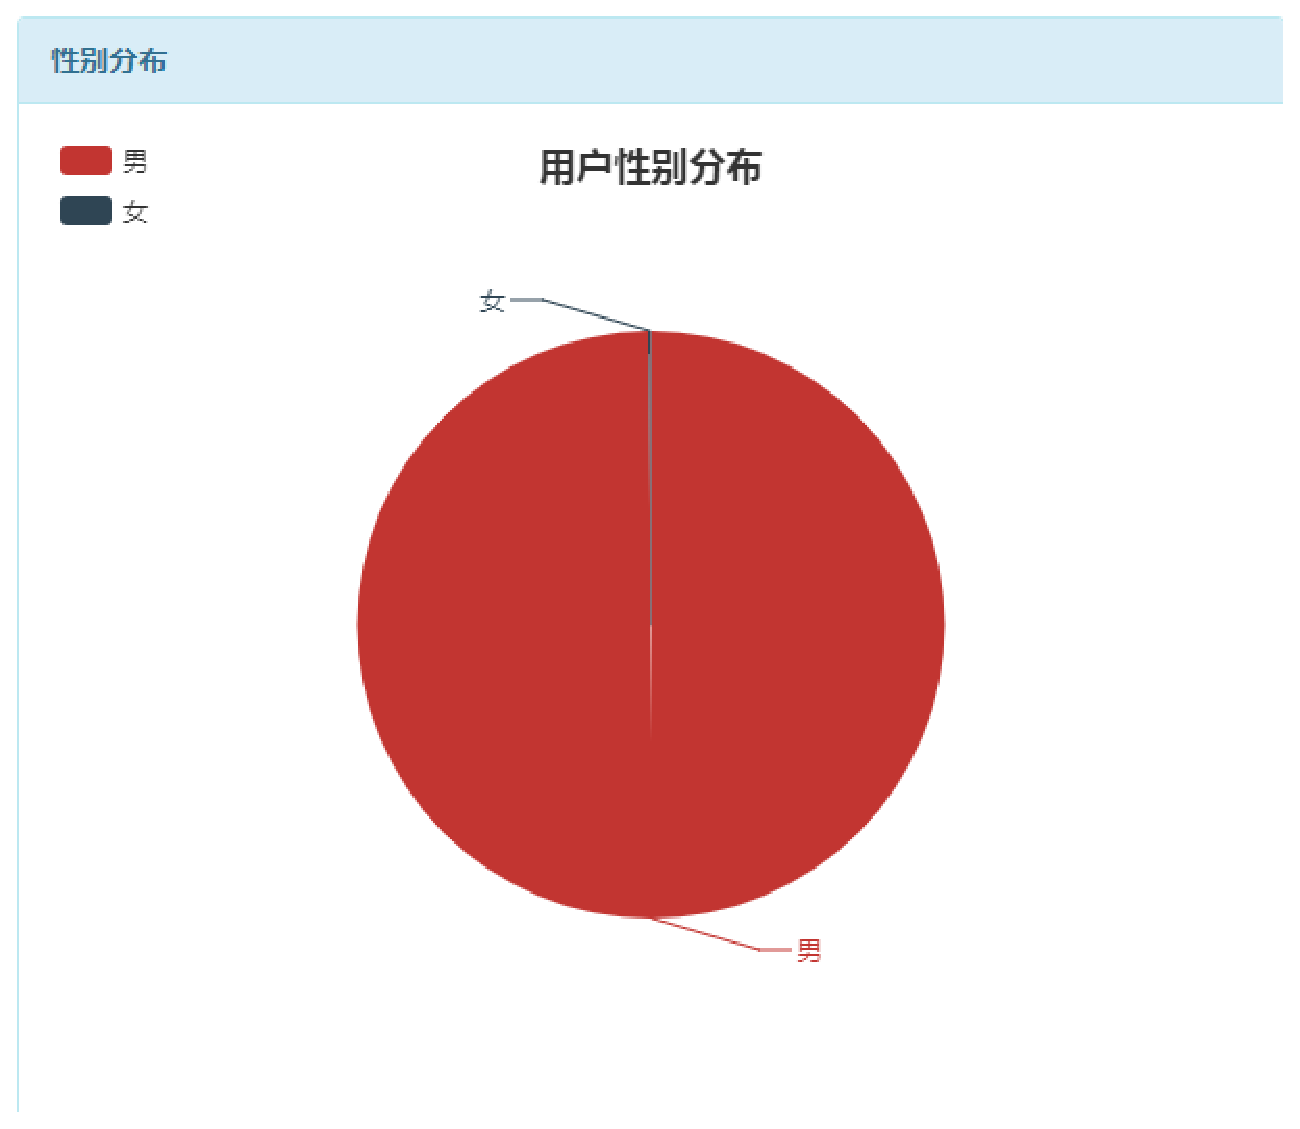
\includegraphics[width=0.15\textwidth]{IMAGE/group-images/11.eps}}
  \subfigure{
      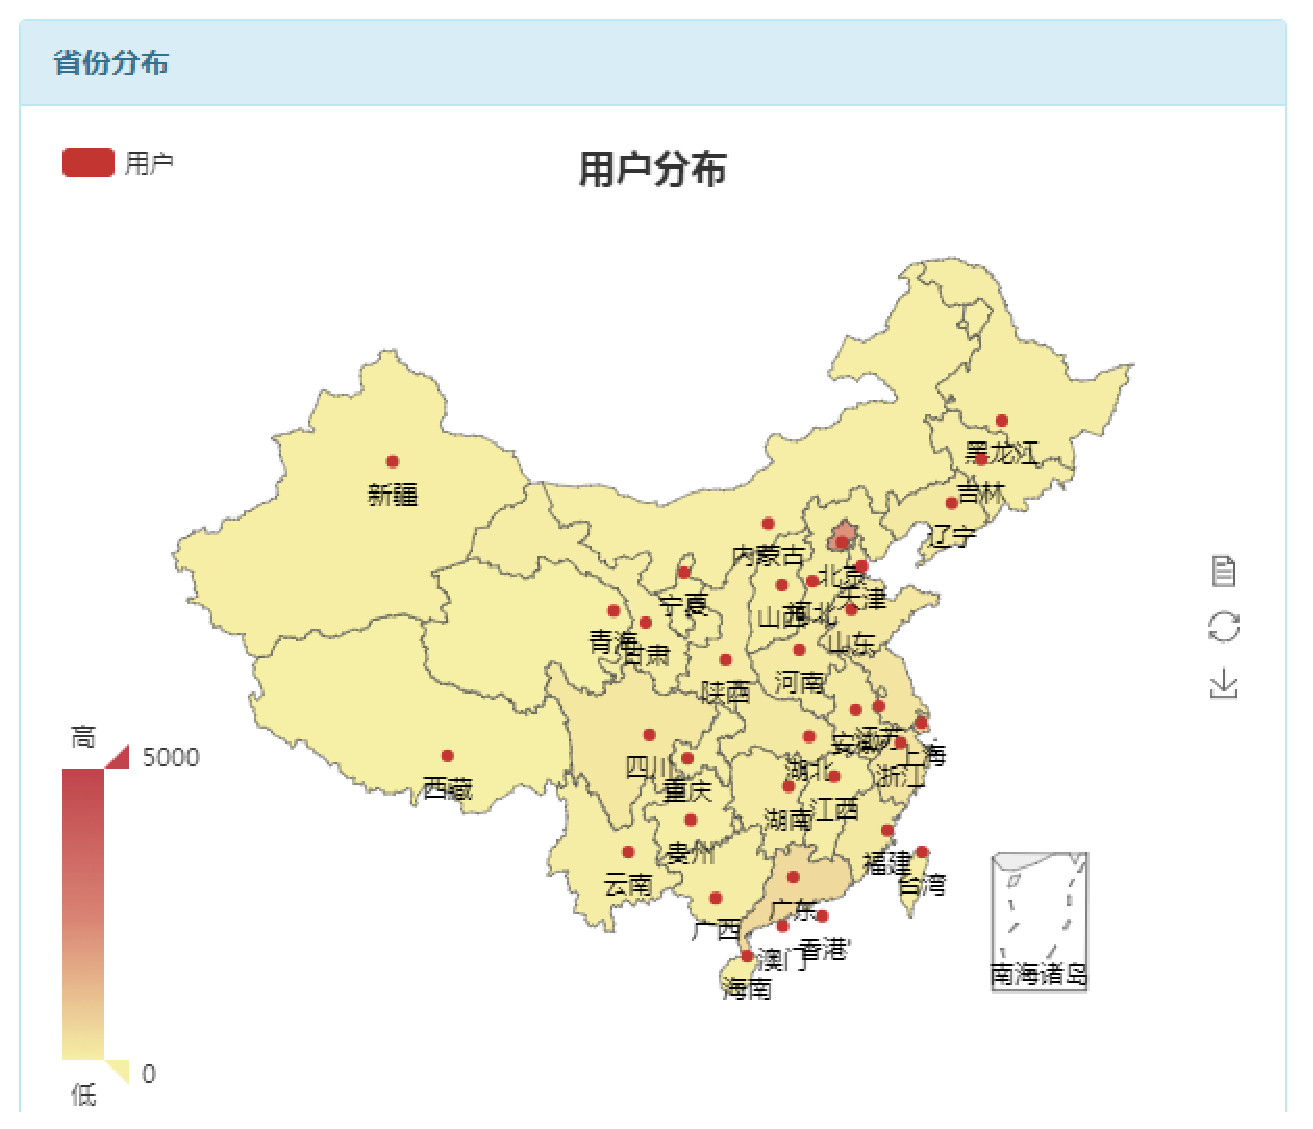
\includegraphics[width=0.15\textwidth]{IMAGE/group-images/12.eps}}
  \subfigure{
      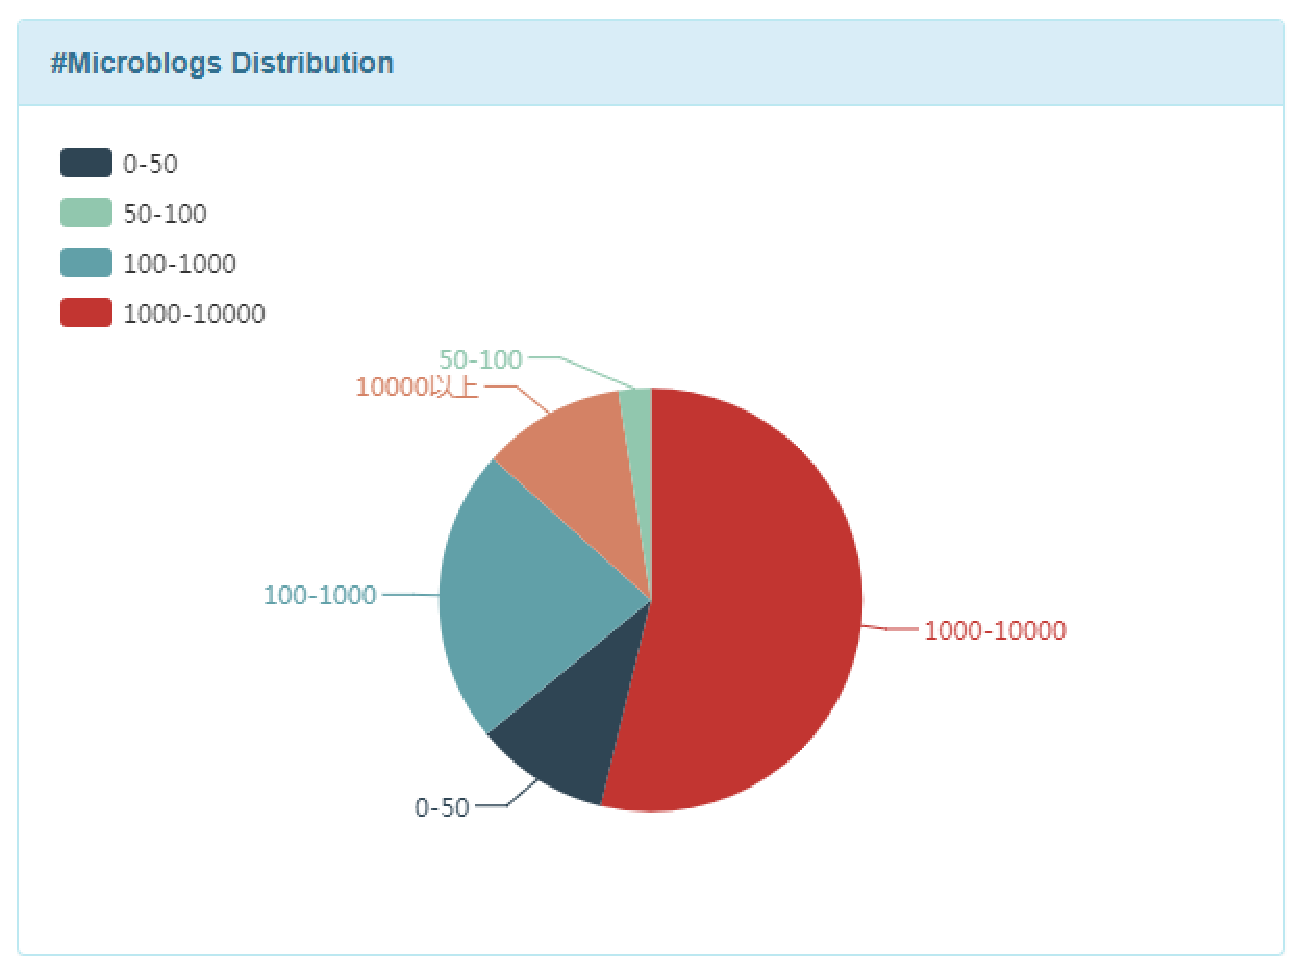
\includegraphics[width=0.15\textwidth]{IMAGE/group-images/13.eps}}
  \subfigure{
      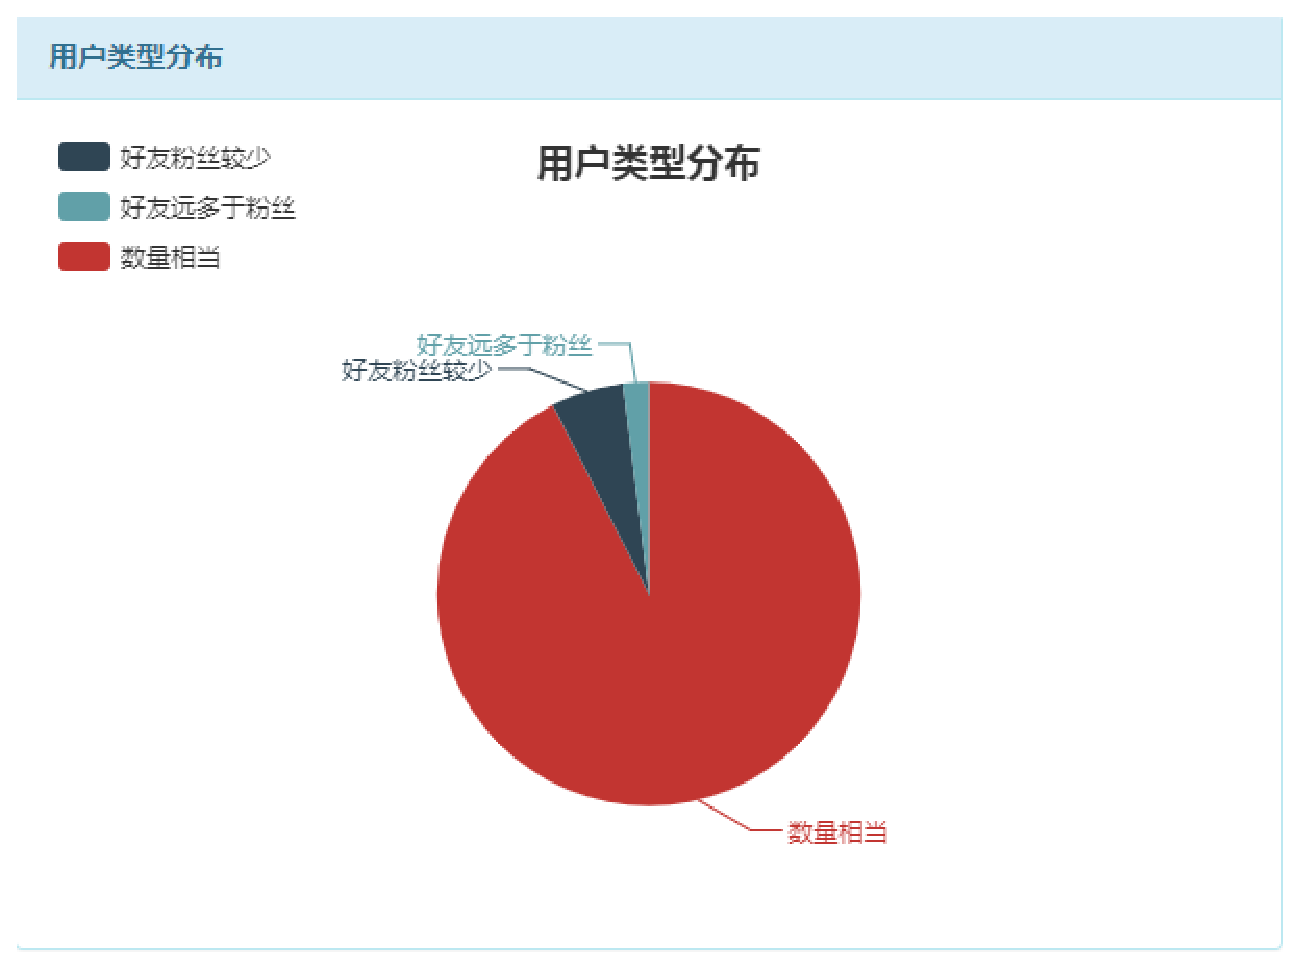
\includegraphics[width=0.15\textwidth]{IMAGE/group-images/14.eps}}
  \subfigure{
      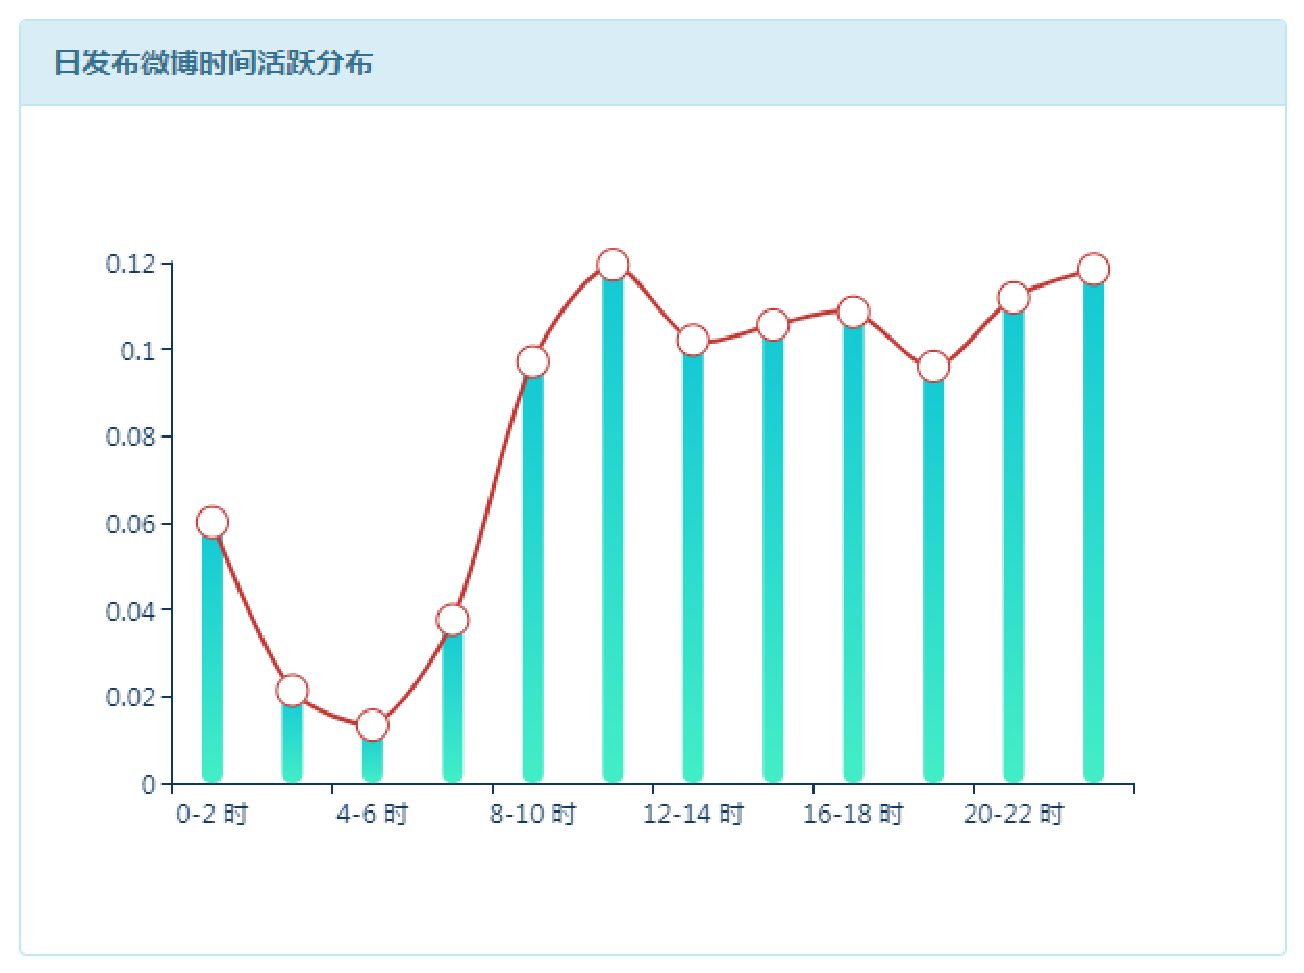
\includegraphics[width=0.15\textwidth]{IMAGE/group-images/15.eps}}
  \subfigure{
      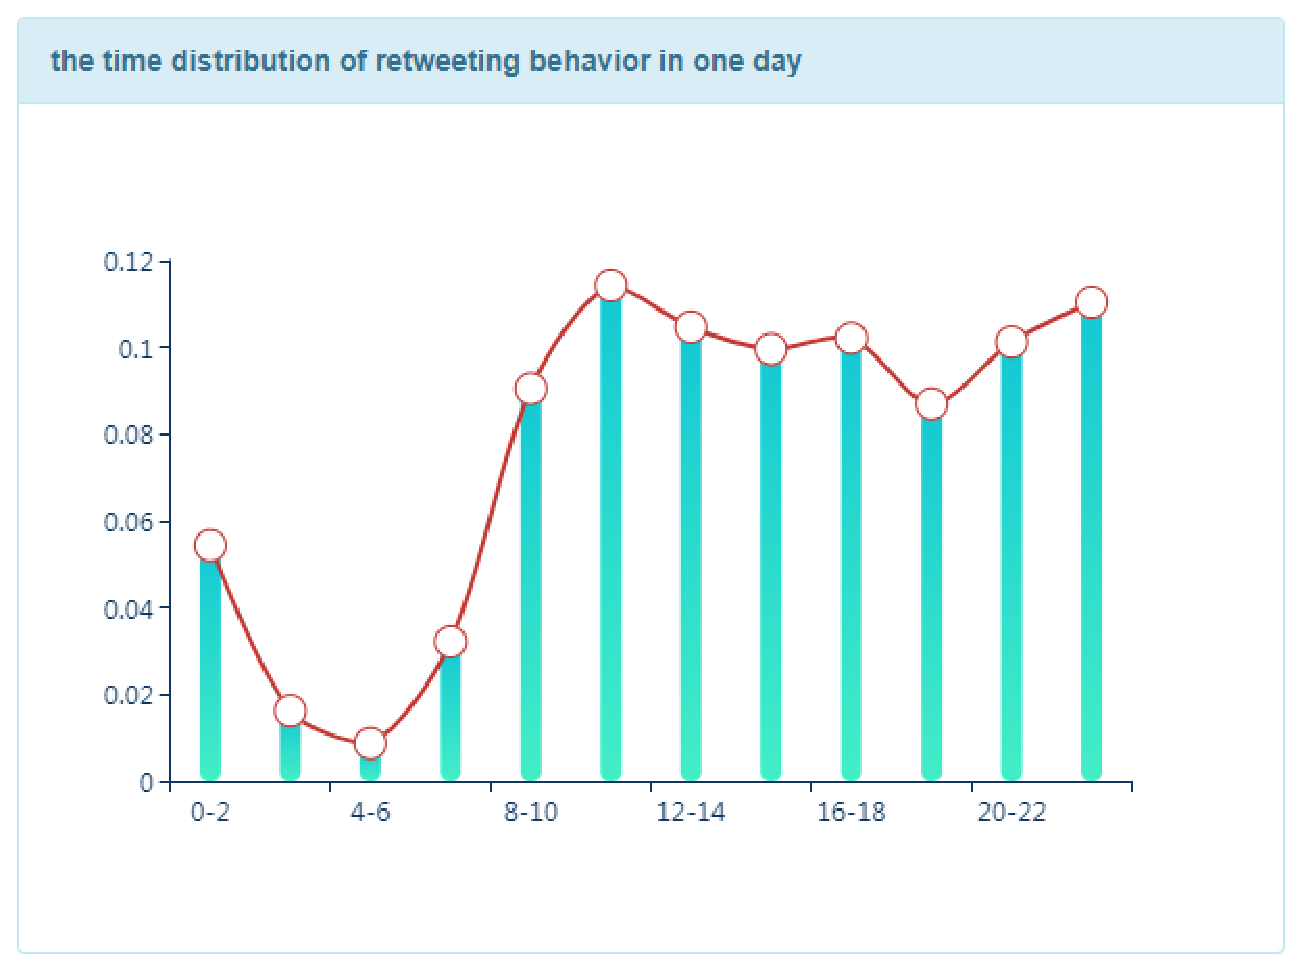
\includegraphics[width=0.15\textwidth]{IMAGE/group-images/16.eps}}
  \subfigure{
      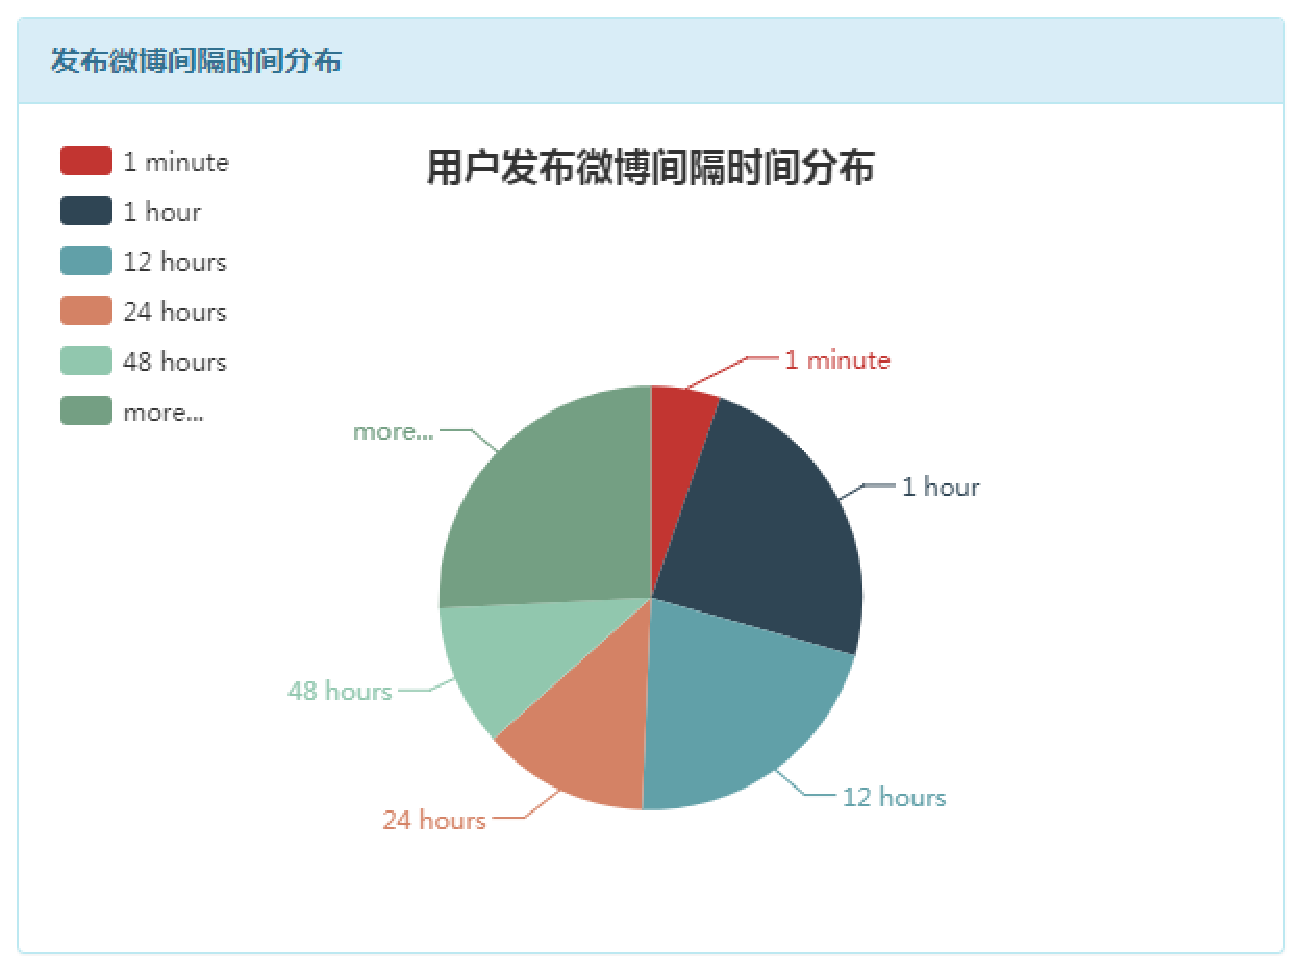
\includegraphics[width=0.15\textwidth]{IMAGE/group-images/17.eps}}
  \subfigure{
      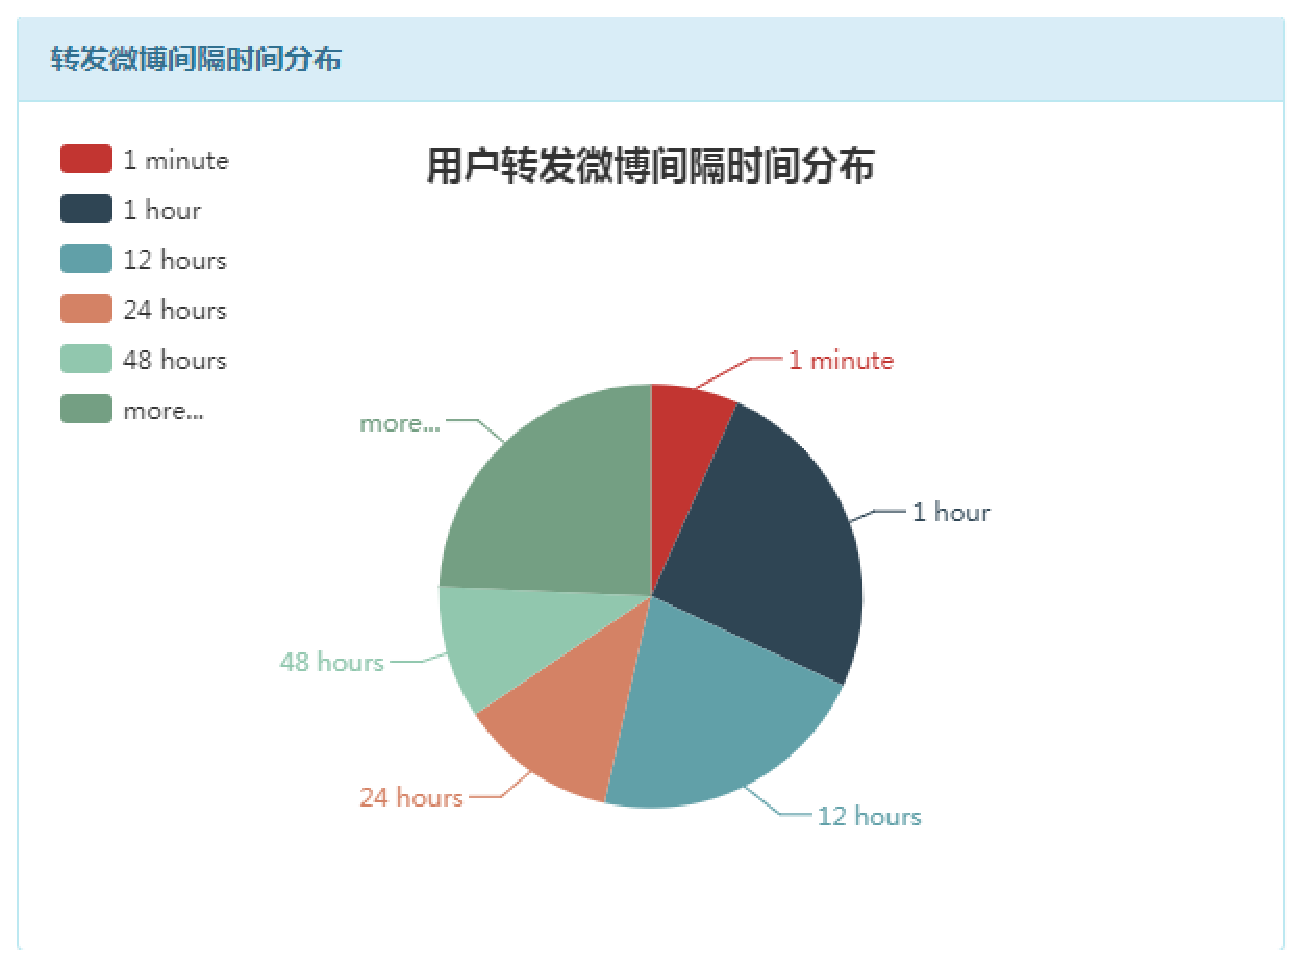
\includegraphics[width=0.15\textwidth]{IMAGE/group-images/18.eps}}
  \subfigure{
      
\includegraphics[width=0.15\textwidth]{IMAGE/group-images/19.eps}}
  \caption{The Statistics of User Group One}
  \label{fig:subfig1} %% label for entire figure
\end{figure}

\begin{figure}
  \centering
  \subfigure{
      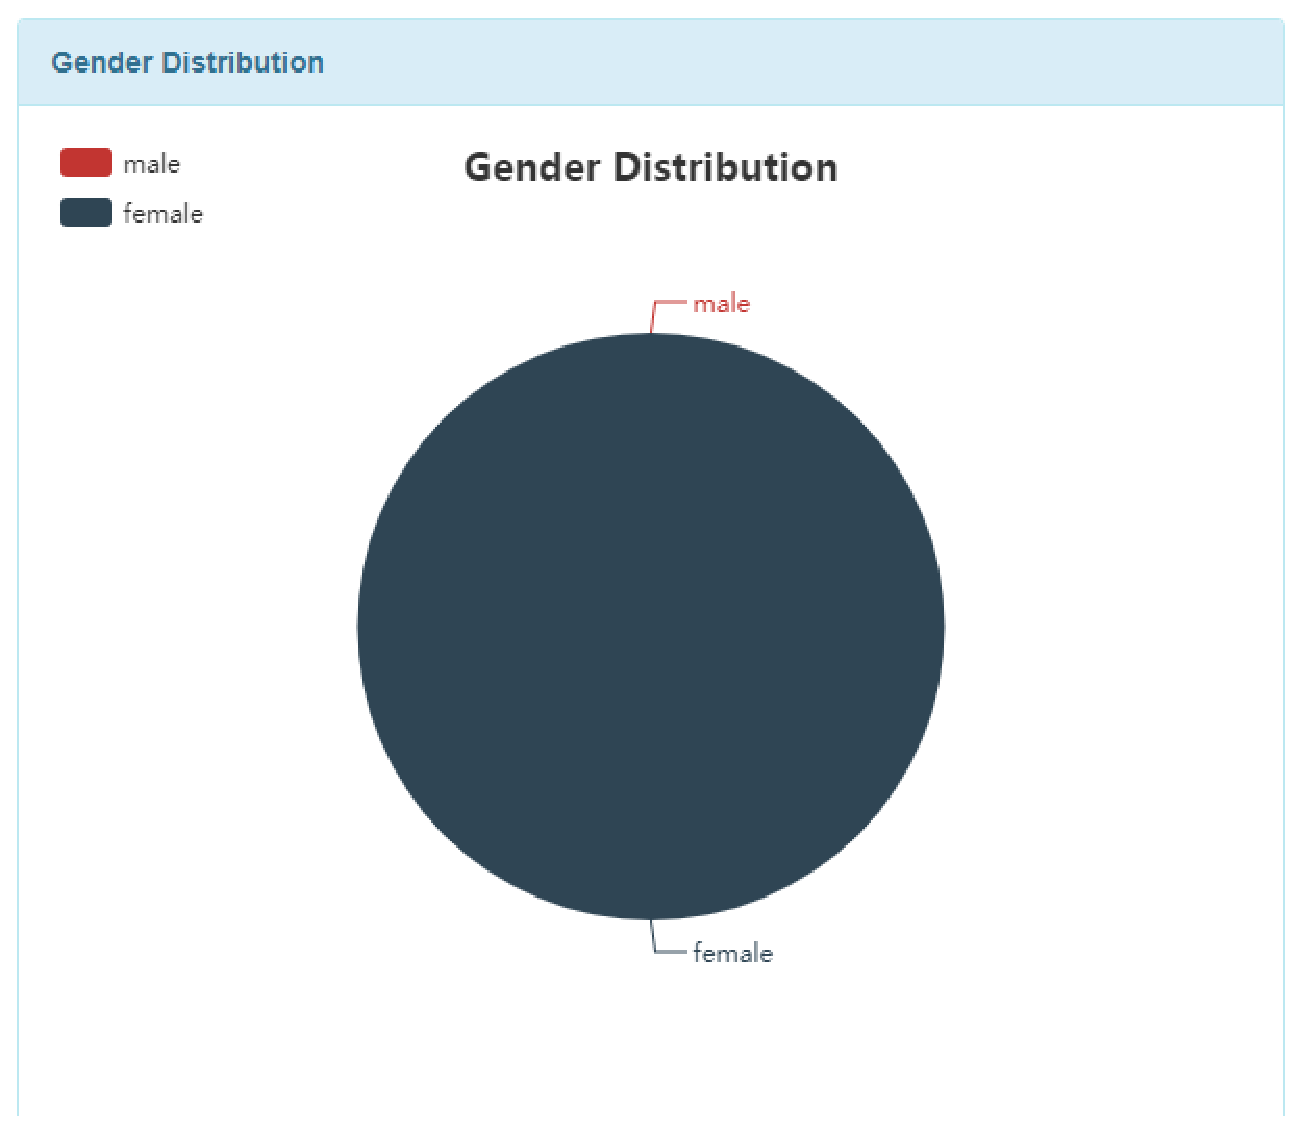
\includegraphics[width=0.15\textwidth]{IMAGE/group-images/21.eps}}
  \subfigure{
      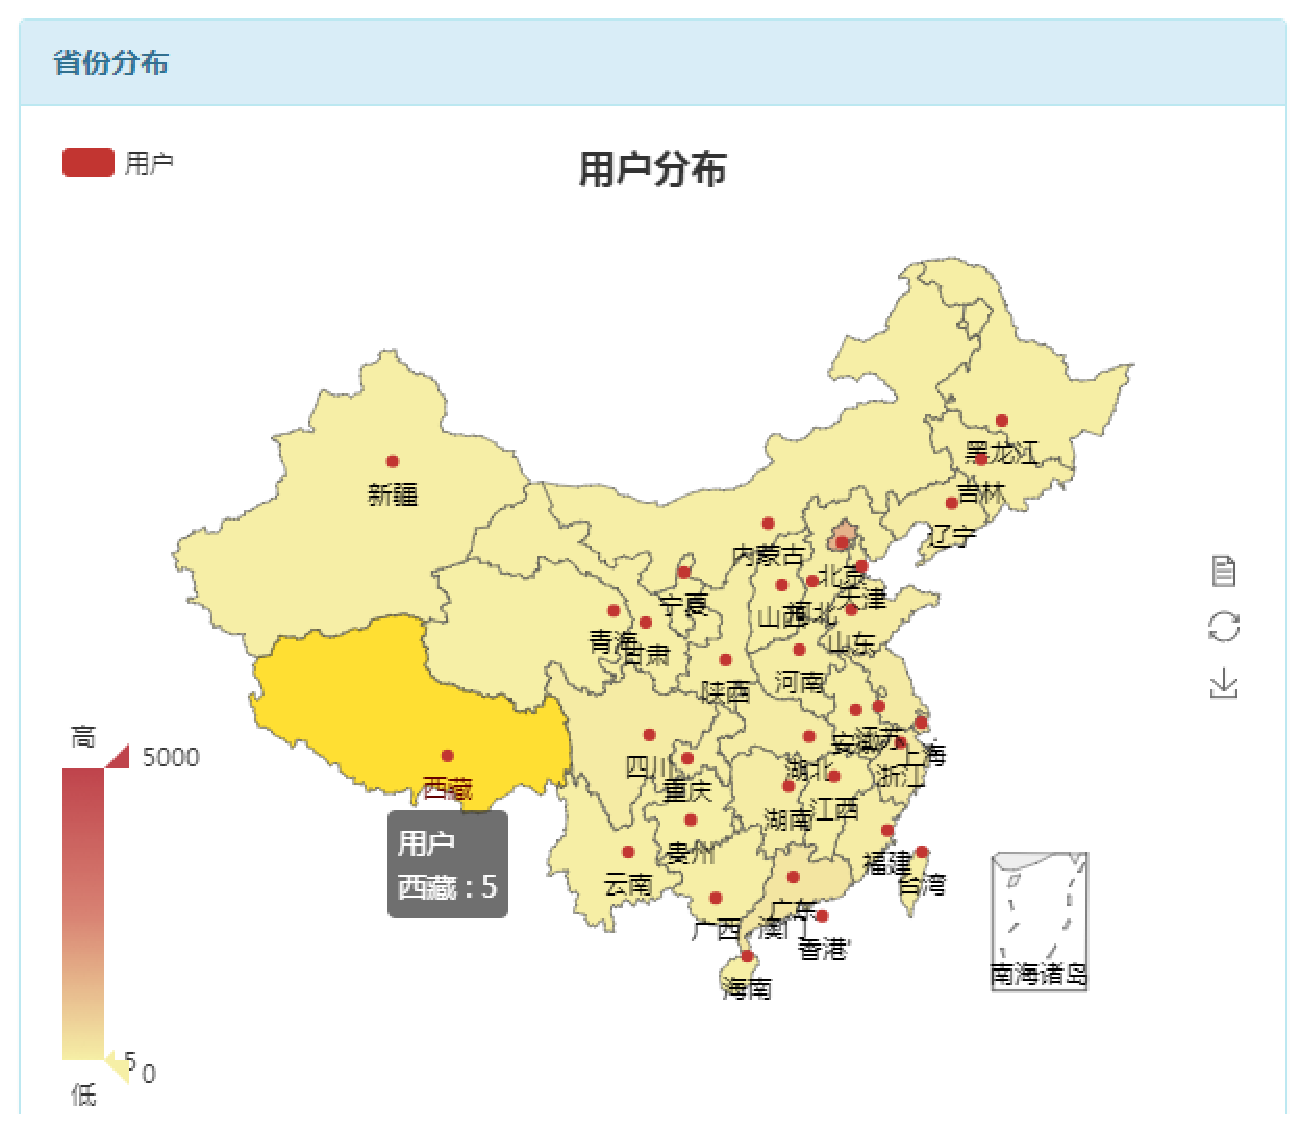
\includegraphics[width=0.15\textwidth]{IMAGE/group-images/22.eps}}
  \subfigure{
      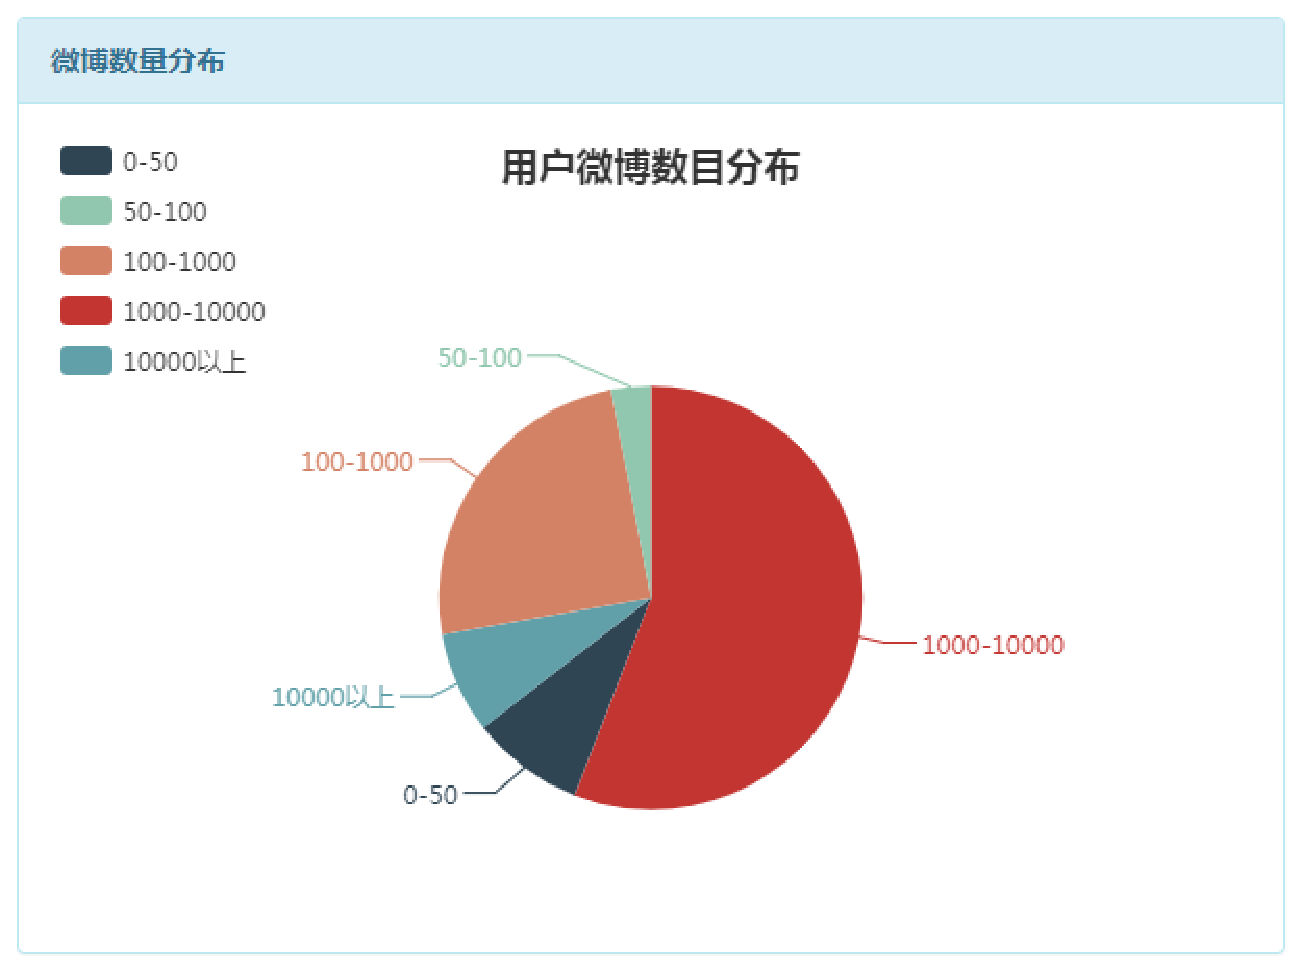
\includegraphics[width=0.15\textwidth]{IMAGE/group-images/23.eps}}
  \subfigure{
      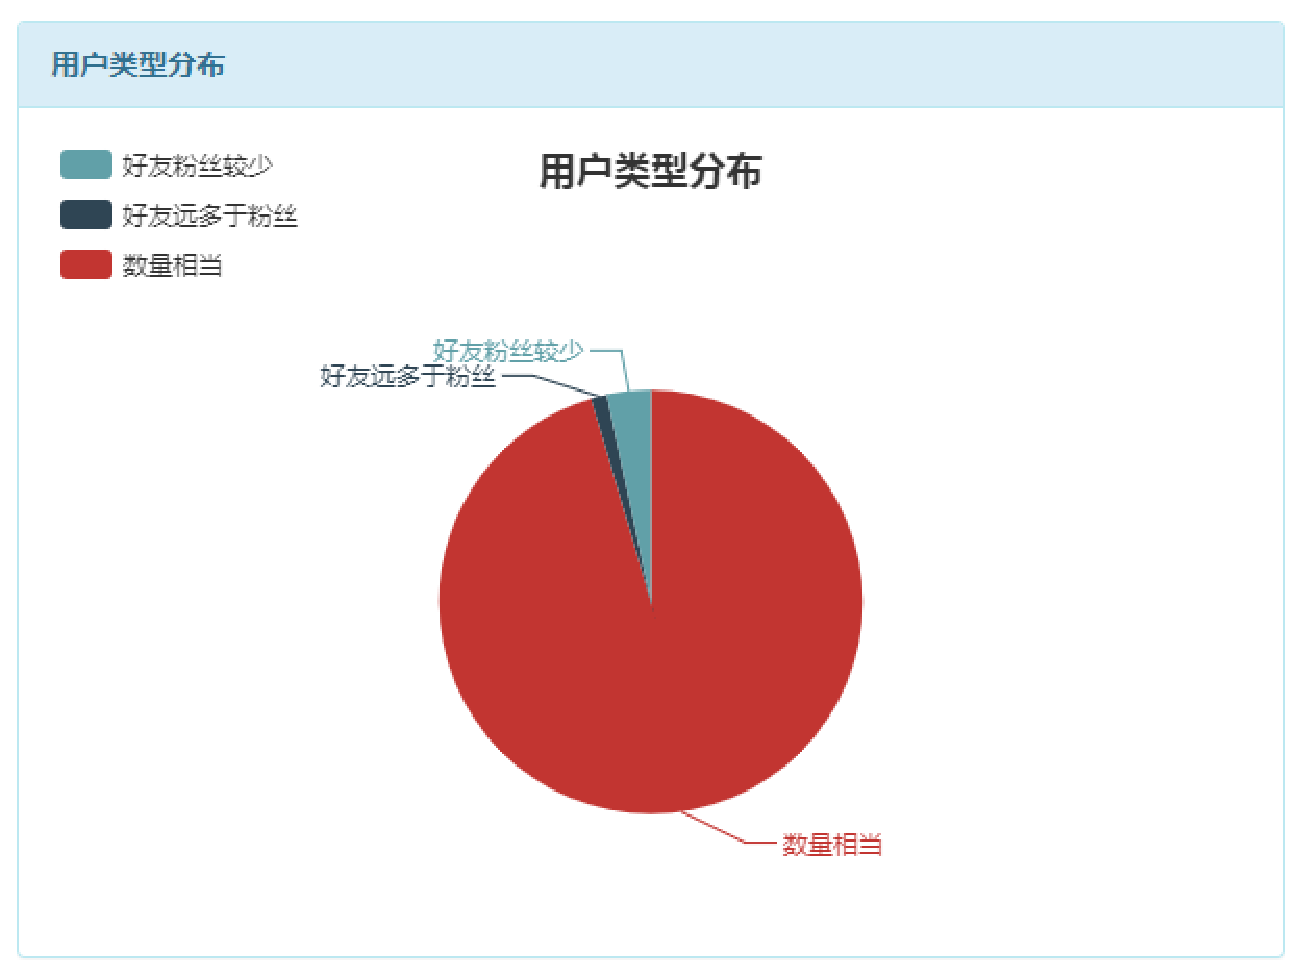
\includegraphics[width=0.15\textwidth]{IMAGE/group-images/24.eps}}
  \subfigure{
      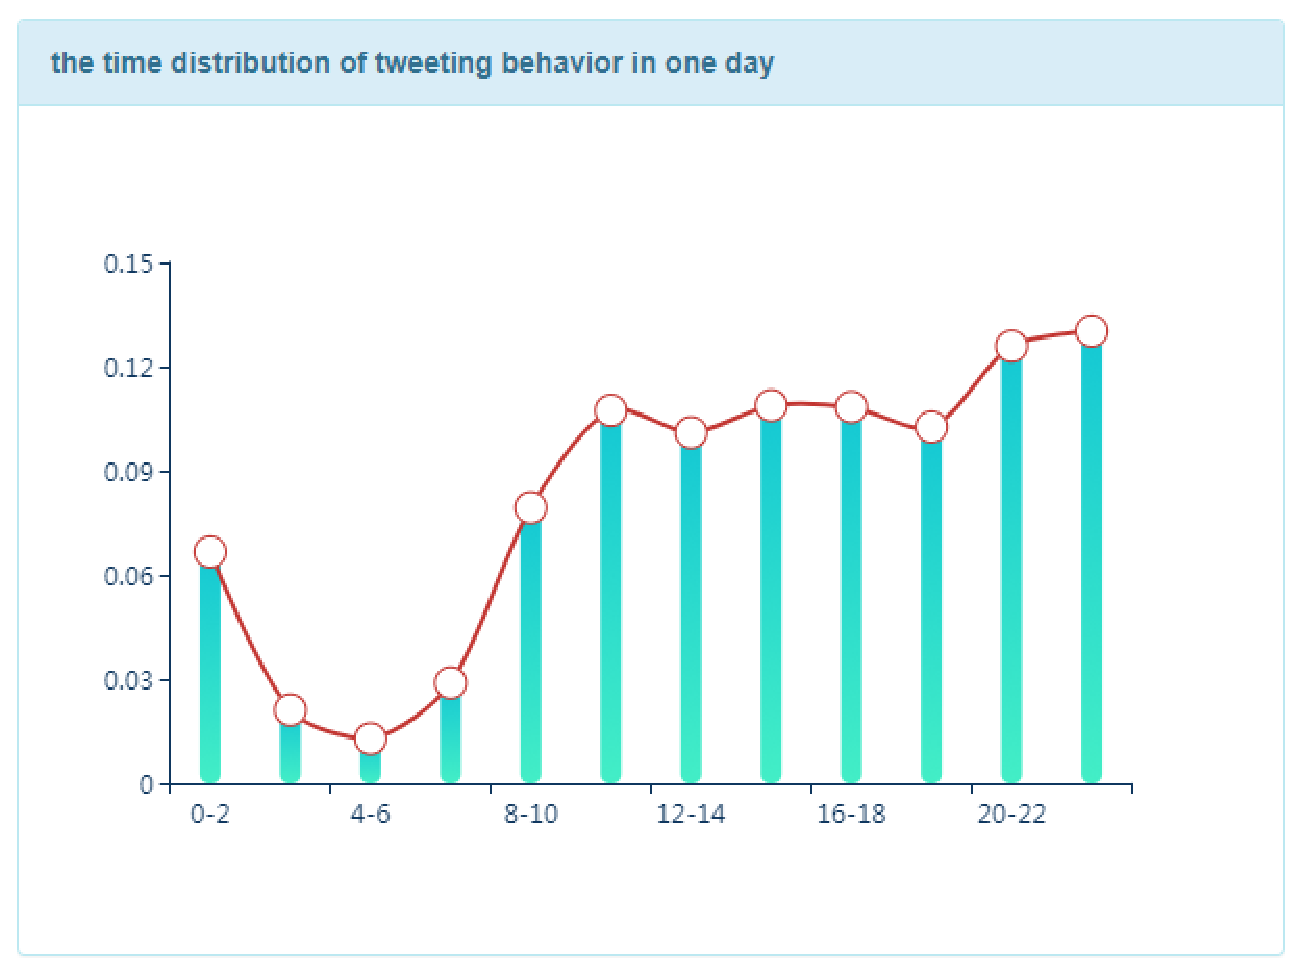
\includegraphics[width=0.15\textwidth]{IMAGE/group-images/25.eps}}
  \subfigure{
      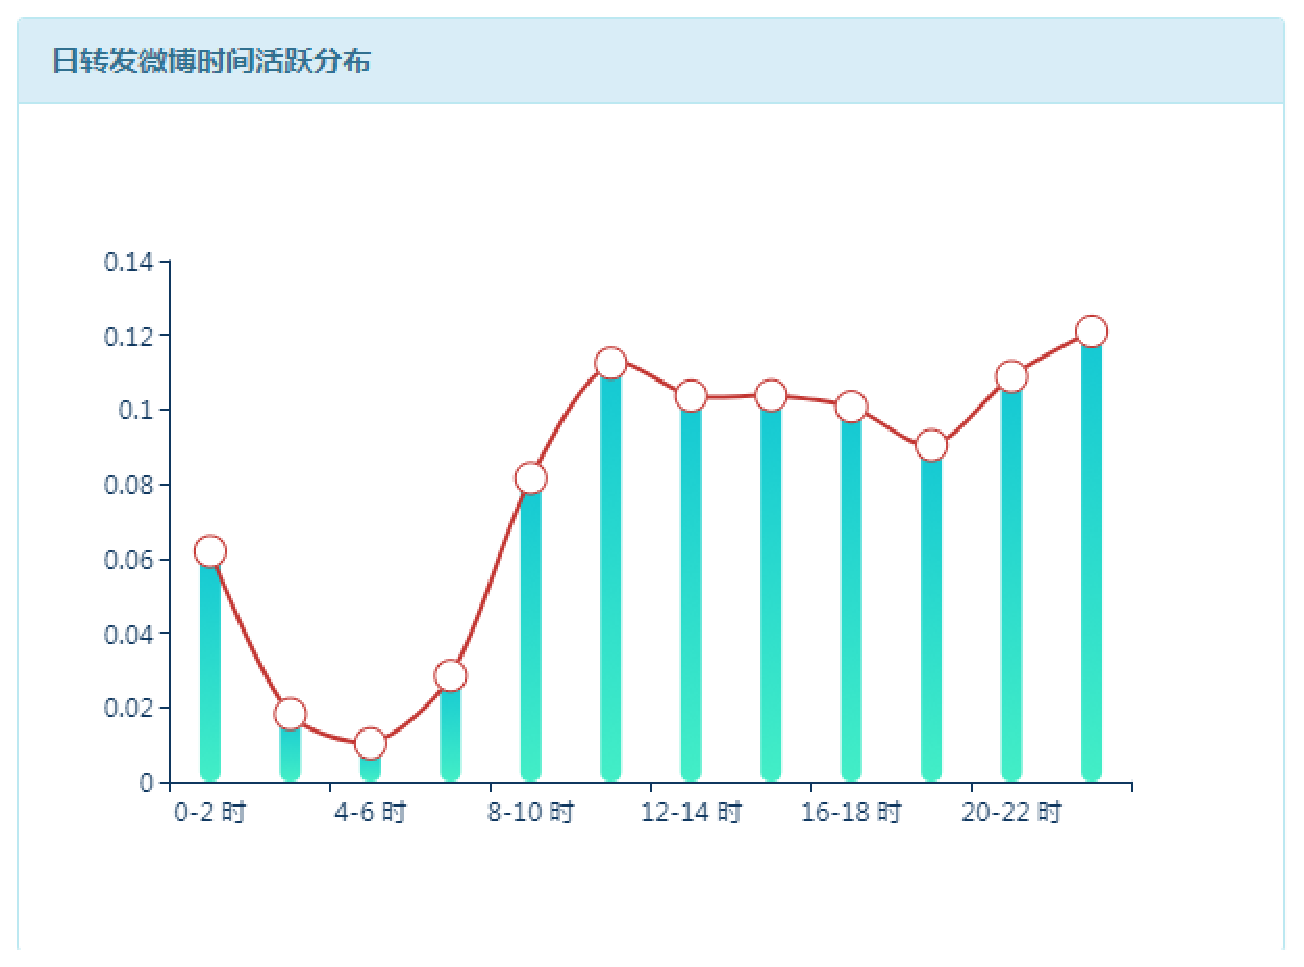
\includegraphics[width=0.15\textwidth]{IMAGE/group-images/26.eps}}
  \subfigure{
      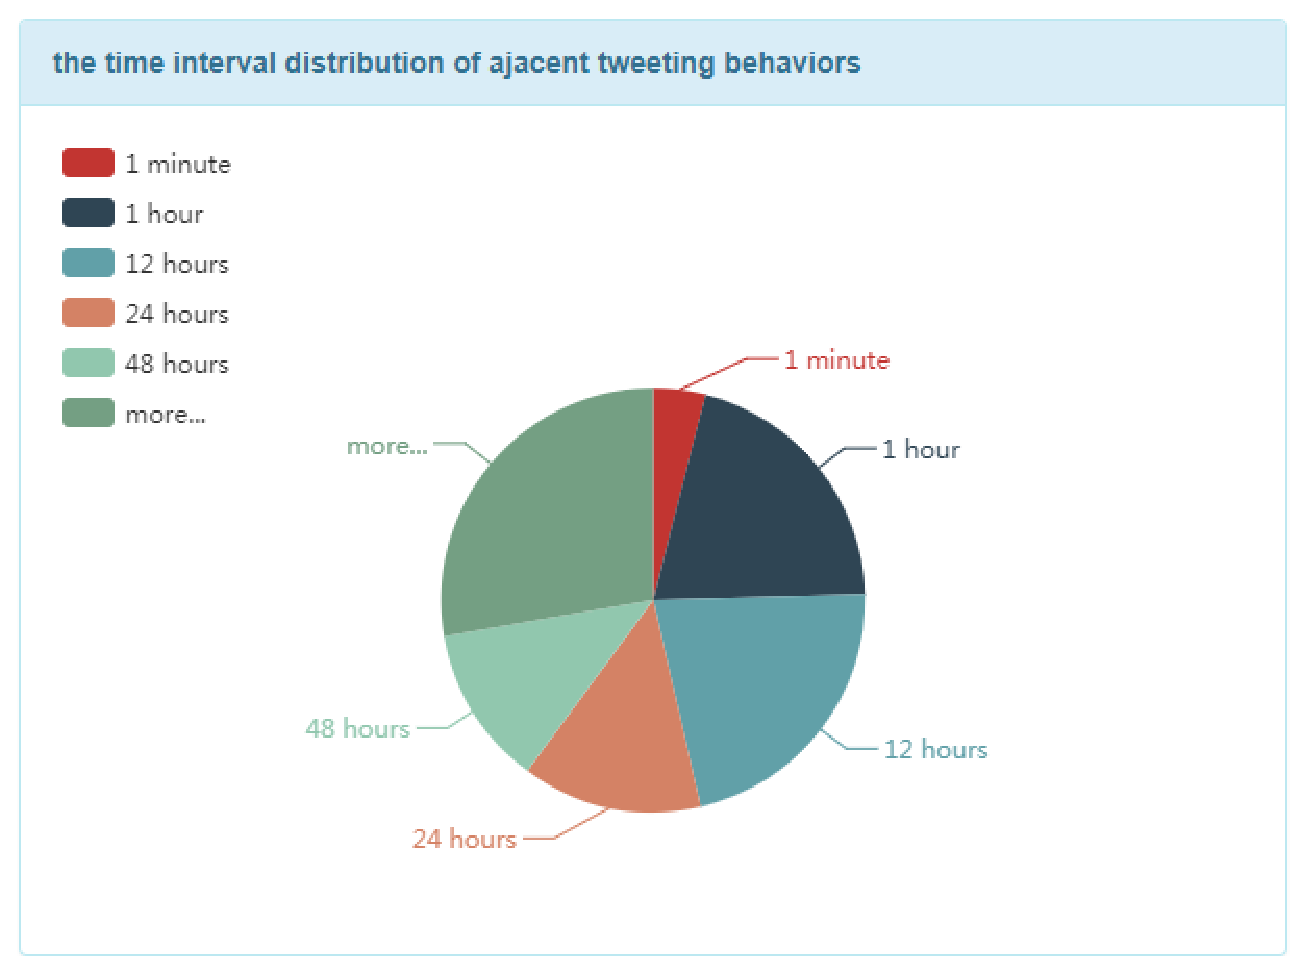
\includegraphics[width=0.15\textwidth]{IMAGE/group-images/27.eps}}
  \subfigure{
      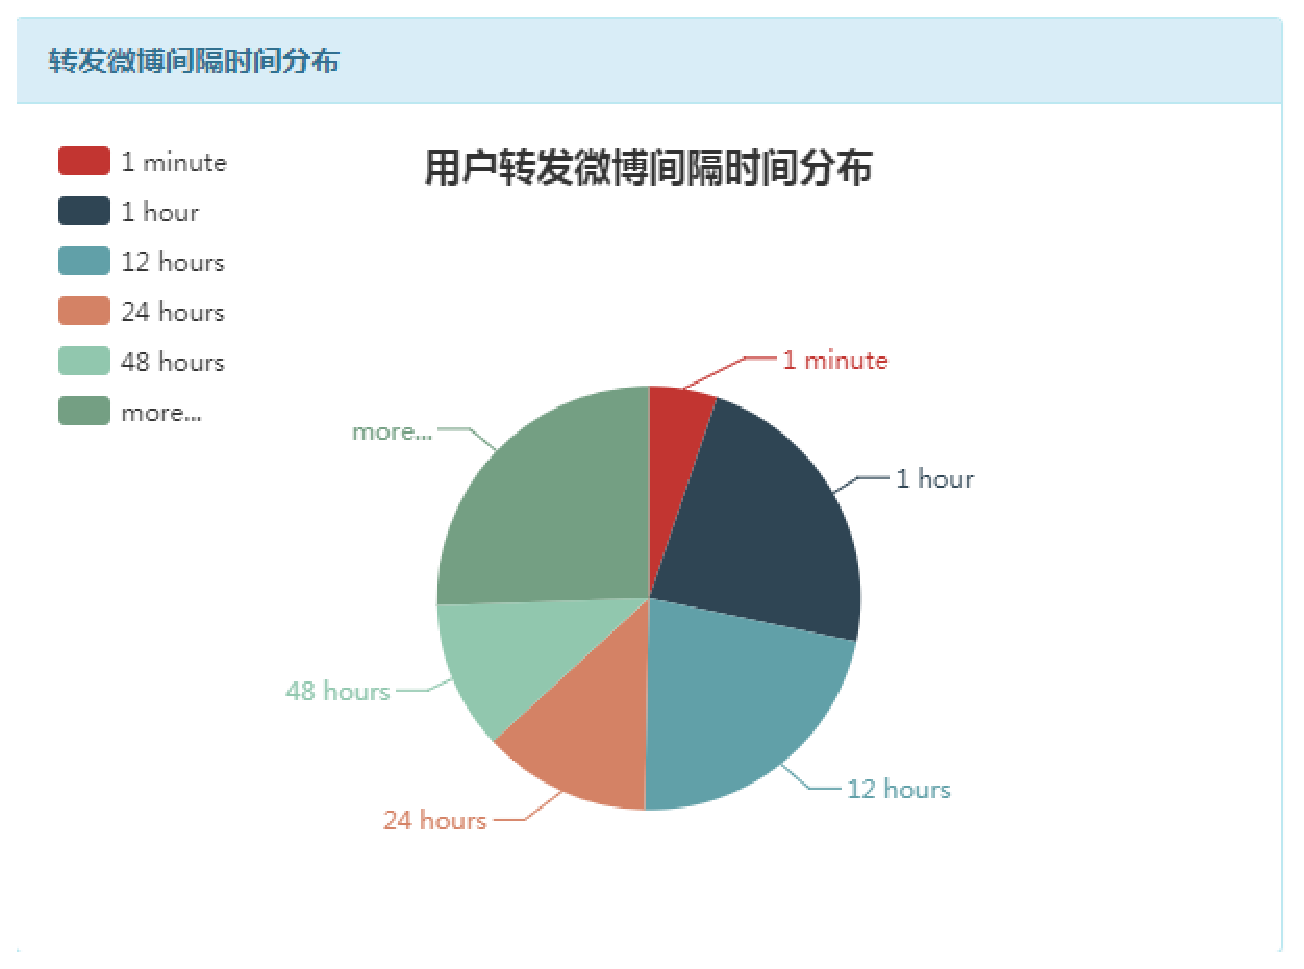
\includegraphics[width=0.15\textwidth]{IMAGE/group-images/28.eps}}
  \subfigure{
      
\includegraphics[width=0.15\textwidth]{IMAGE/group-images/29.eps}}
  \caption{The Statistics of User Group Two}
  \label{fig:subfig2} %% label for entire figure
\end{figure}
\begin{figure}
  \centering
  \subfigure{
      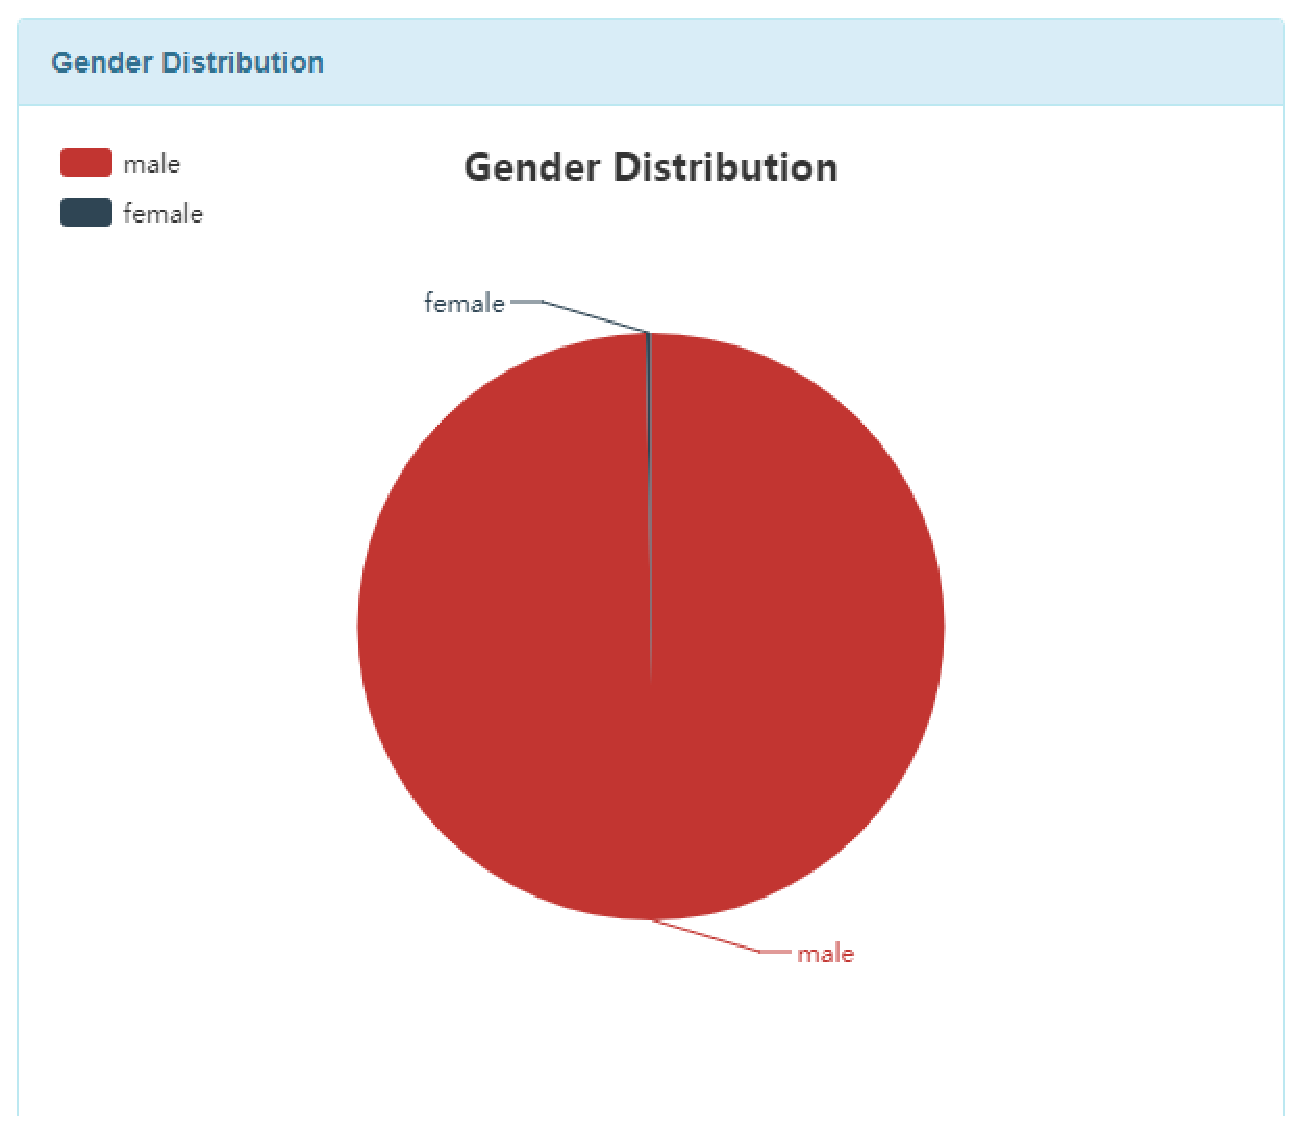
\includegraphics[width=0.15\textwidth]{IMAGE/group-images/31.eps}}
  \subfigure{
      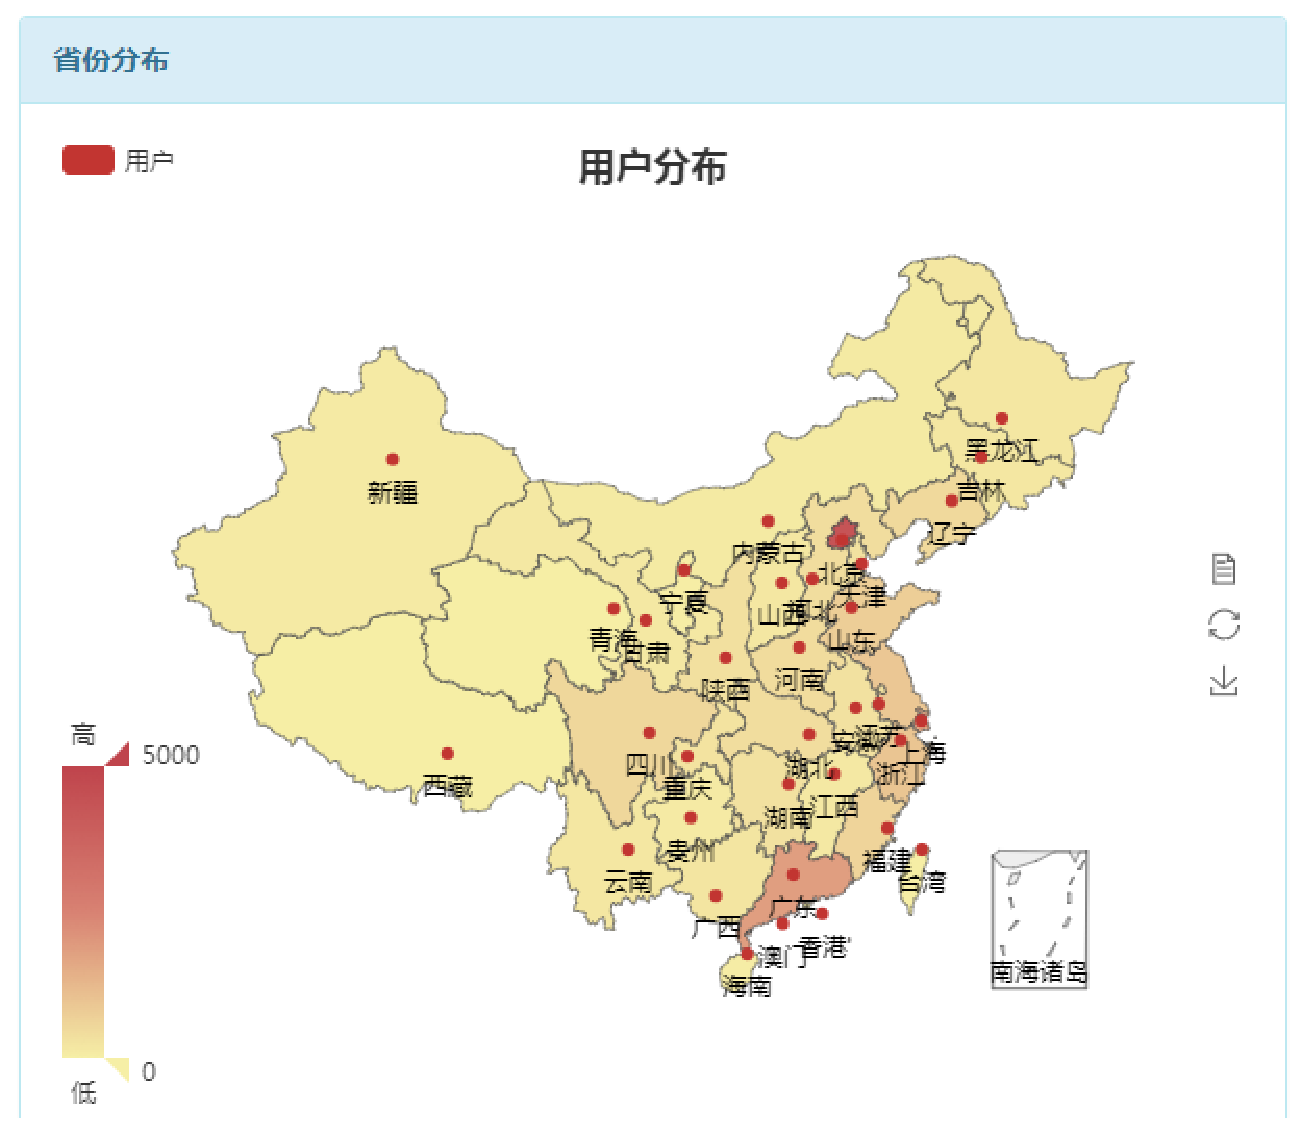
\includegraphics[width=0.15\textwidth]{IMAGE/group-images/32.eps}}
  \subfigure{
      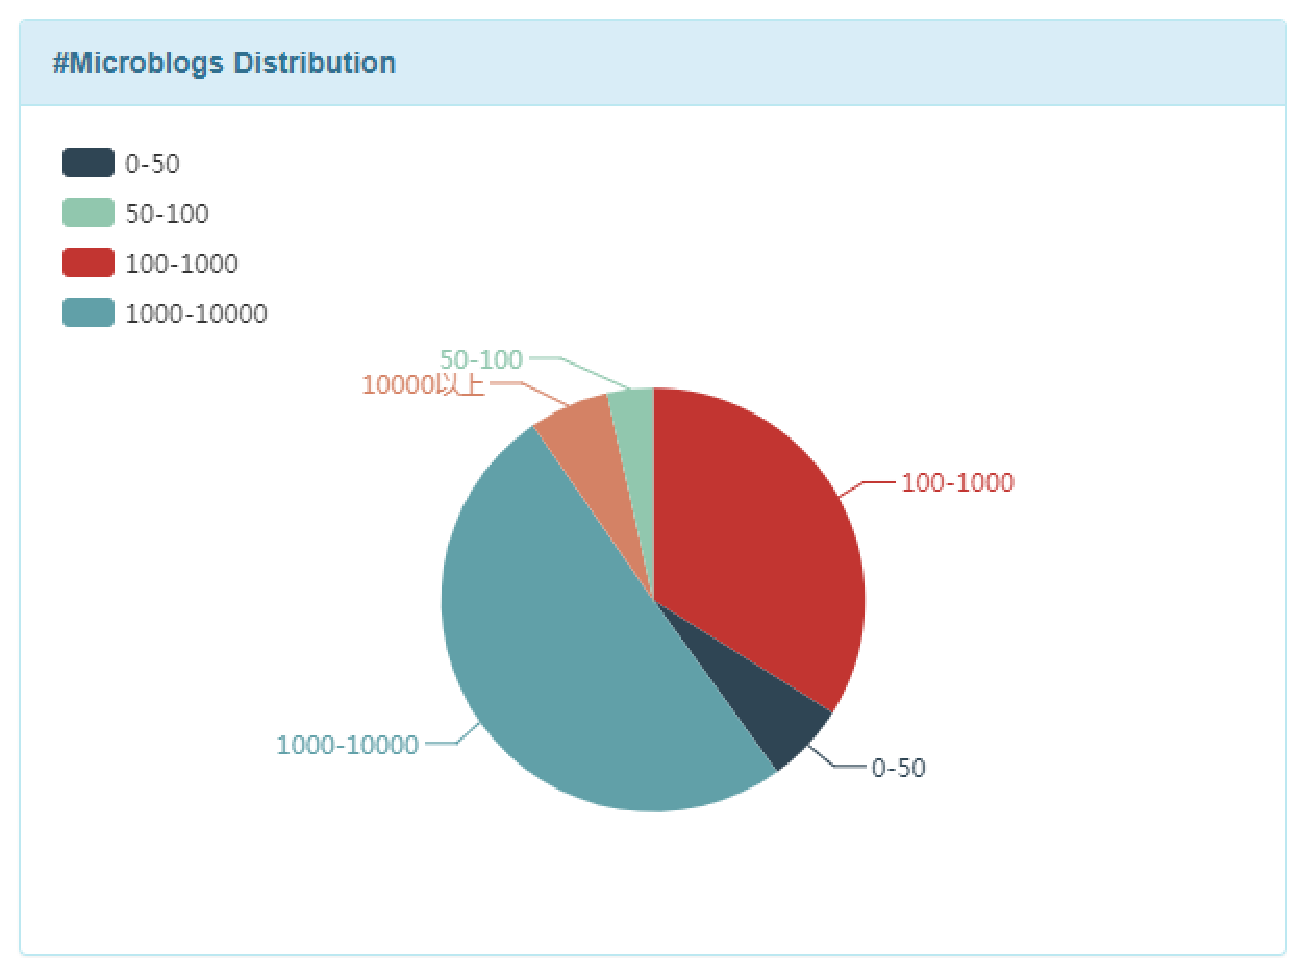
\includegraphics[width=0.15\textwidth]{IMAGE/group-images/33.eps}}
  \subfigure{
      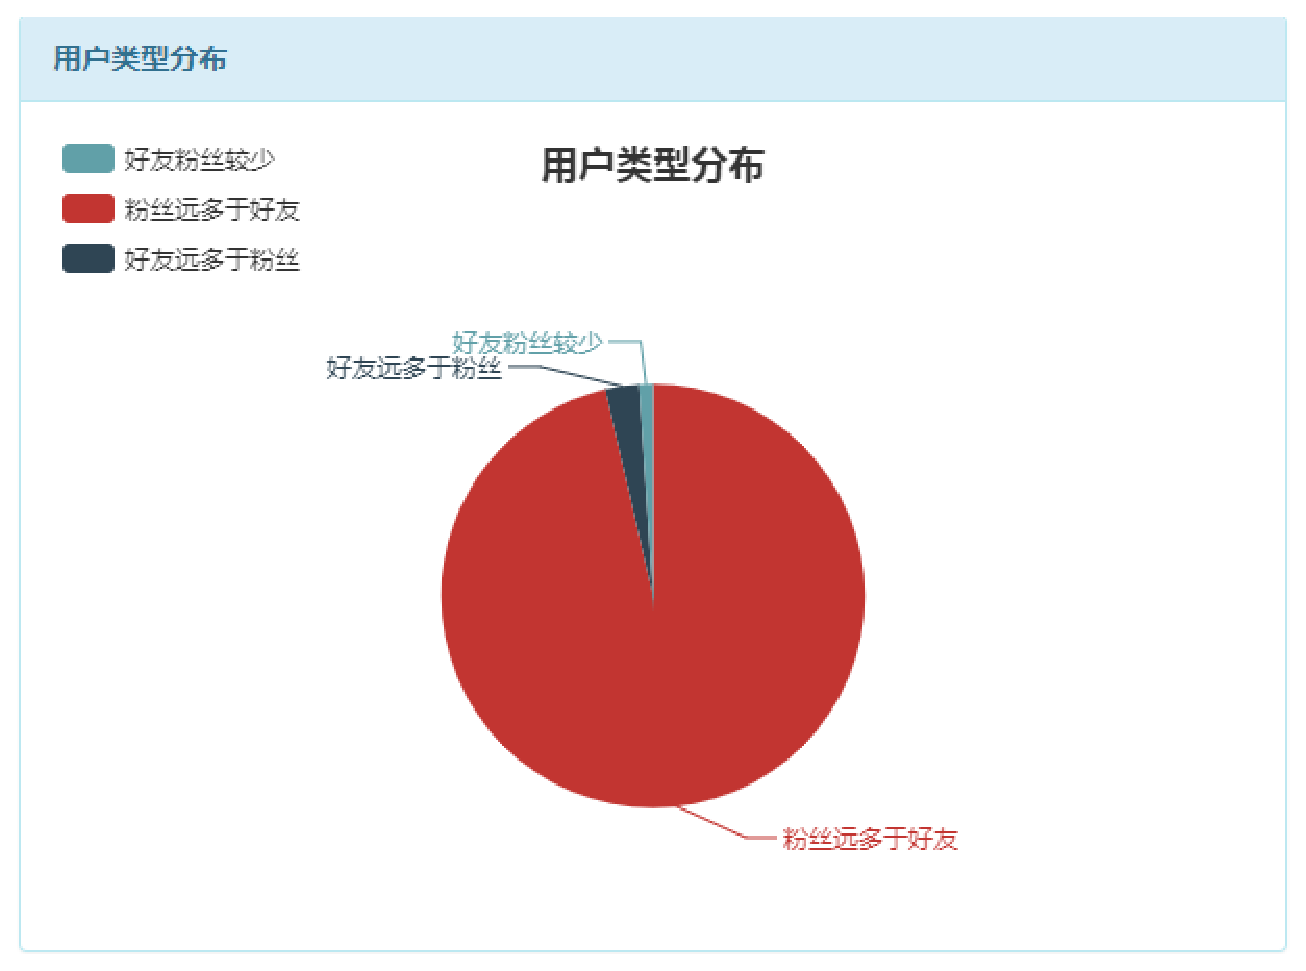
\includegraphics[width=0.15\textwidth]{IMAGE/group-images/34.eps}}
  \subfigure{
      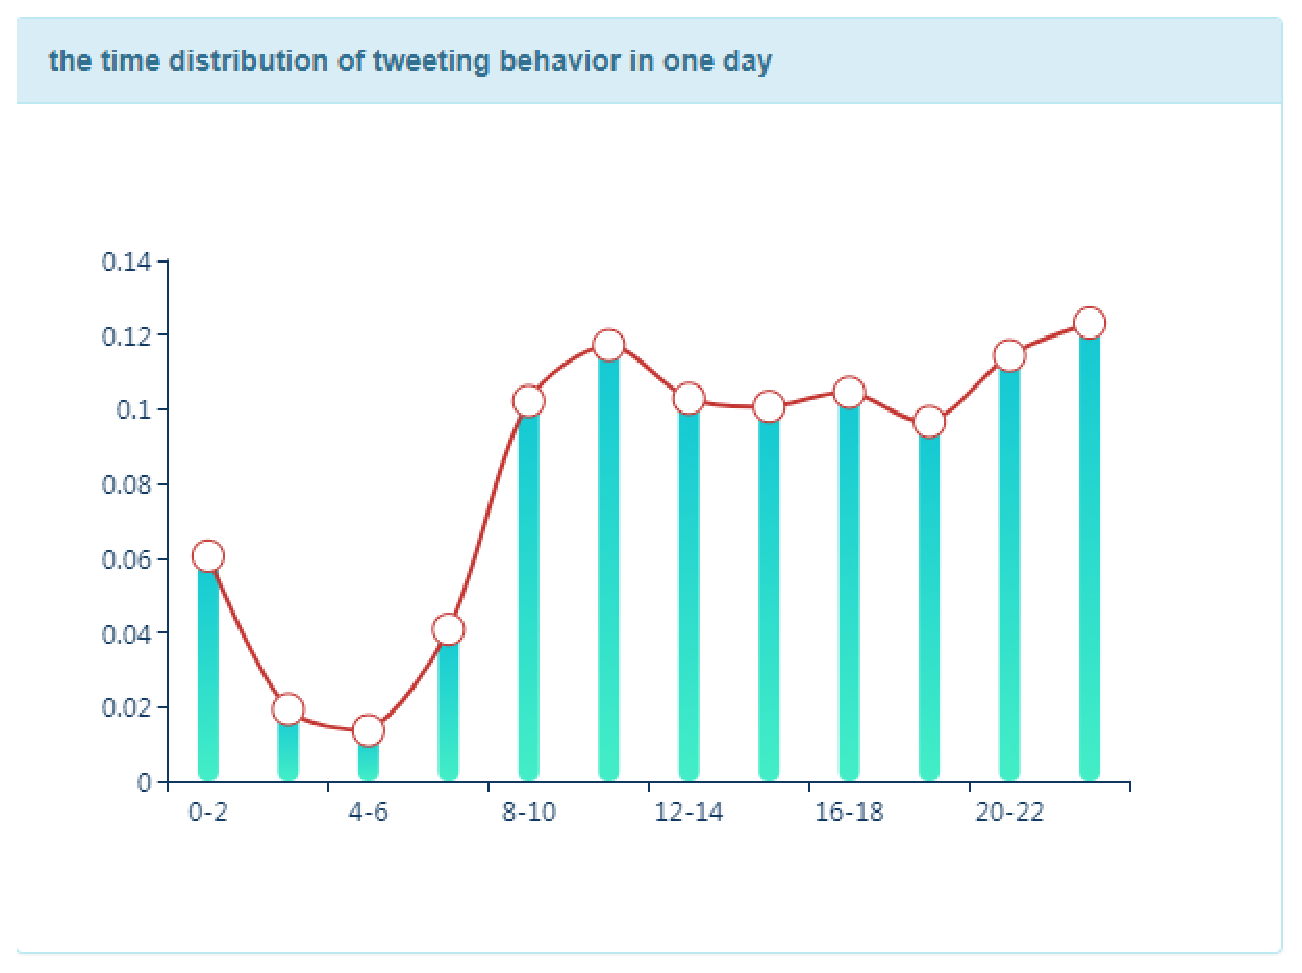
\includegraphics[width=0.15\textwidth]{IMAGE/group-images/35.eps}}
  \subfigure{
      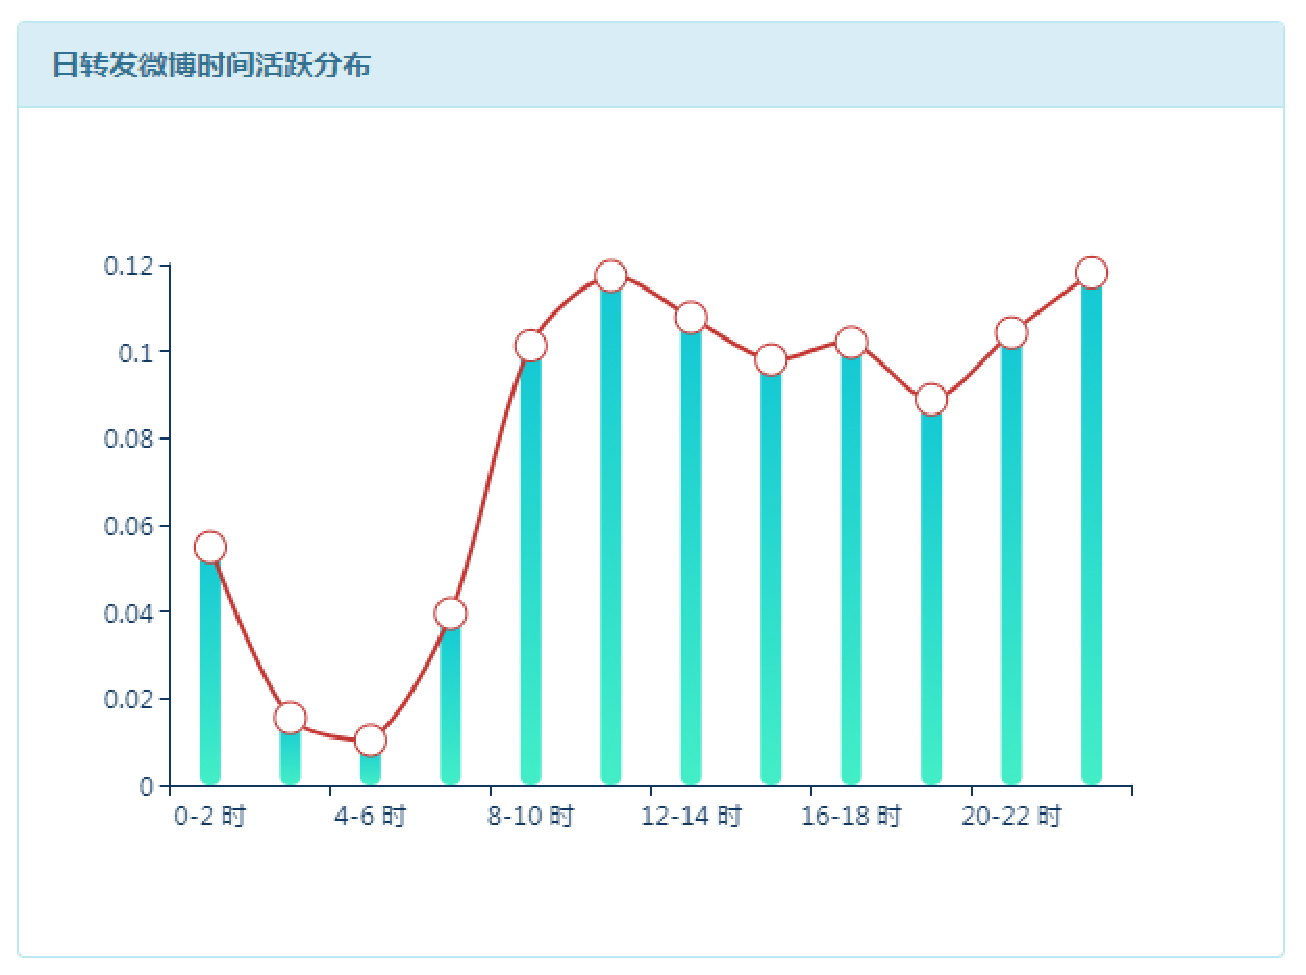
\includegraphics[width=0.15\textwidth]{IMAGE/group-images/36.eps}}
  \subfigure{
      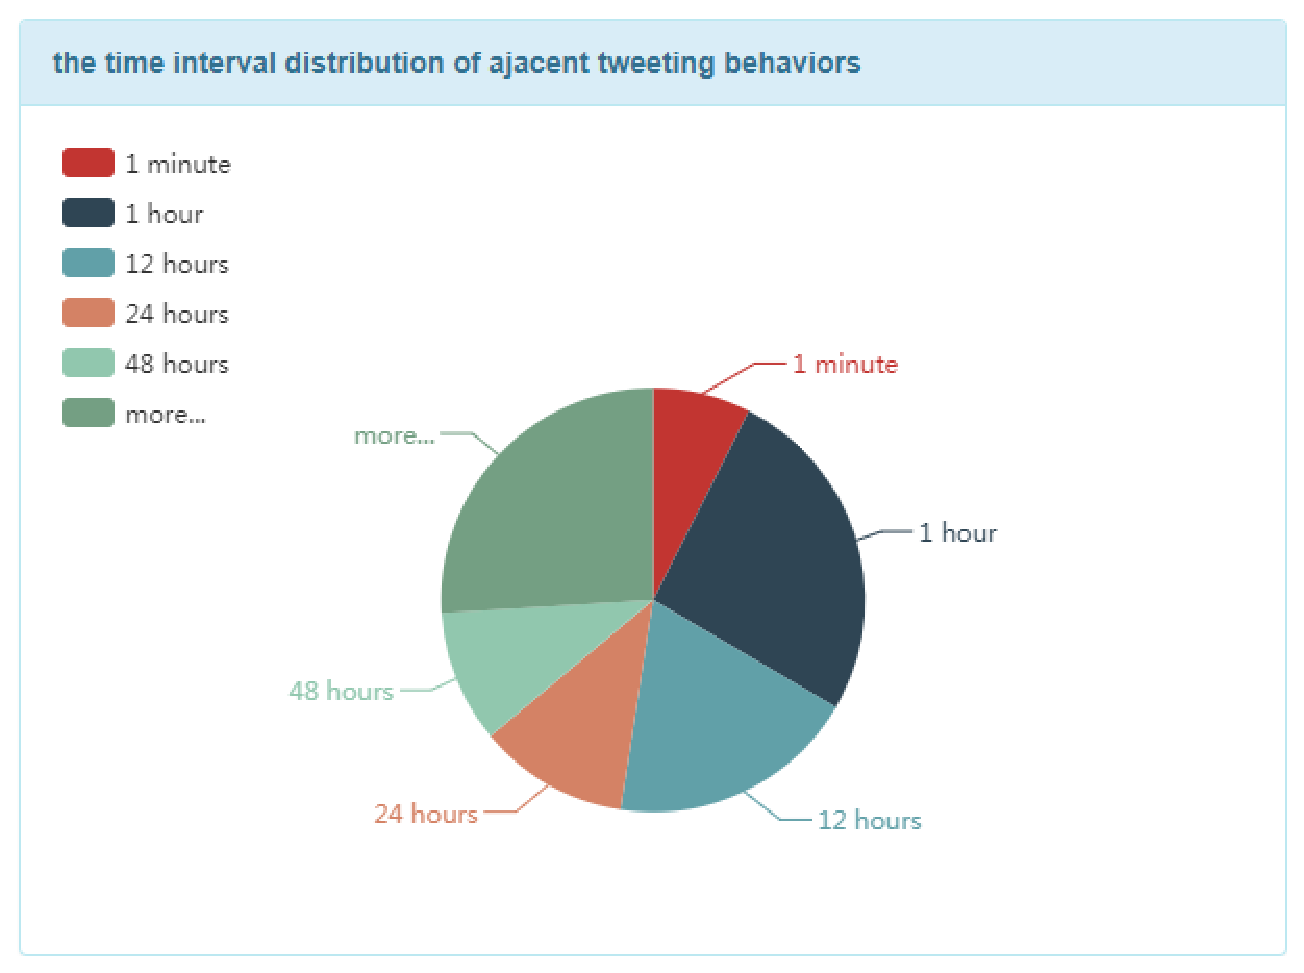
\includegraphics[width=0.15\textwidth]{IMAGE/group-images/37.eps}}
  \subfigure{
      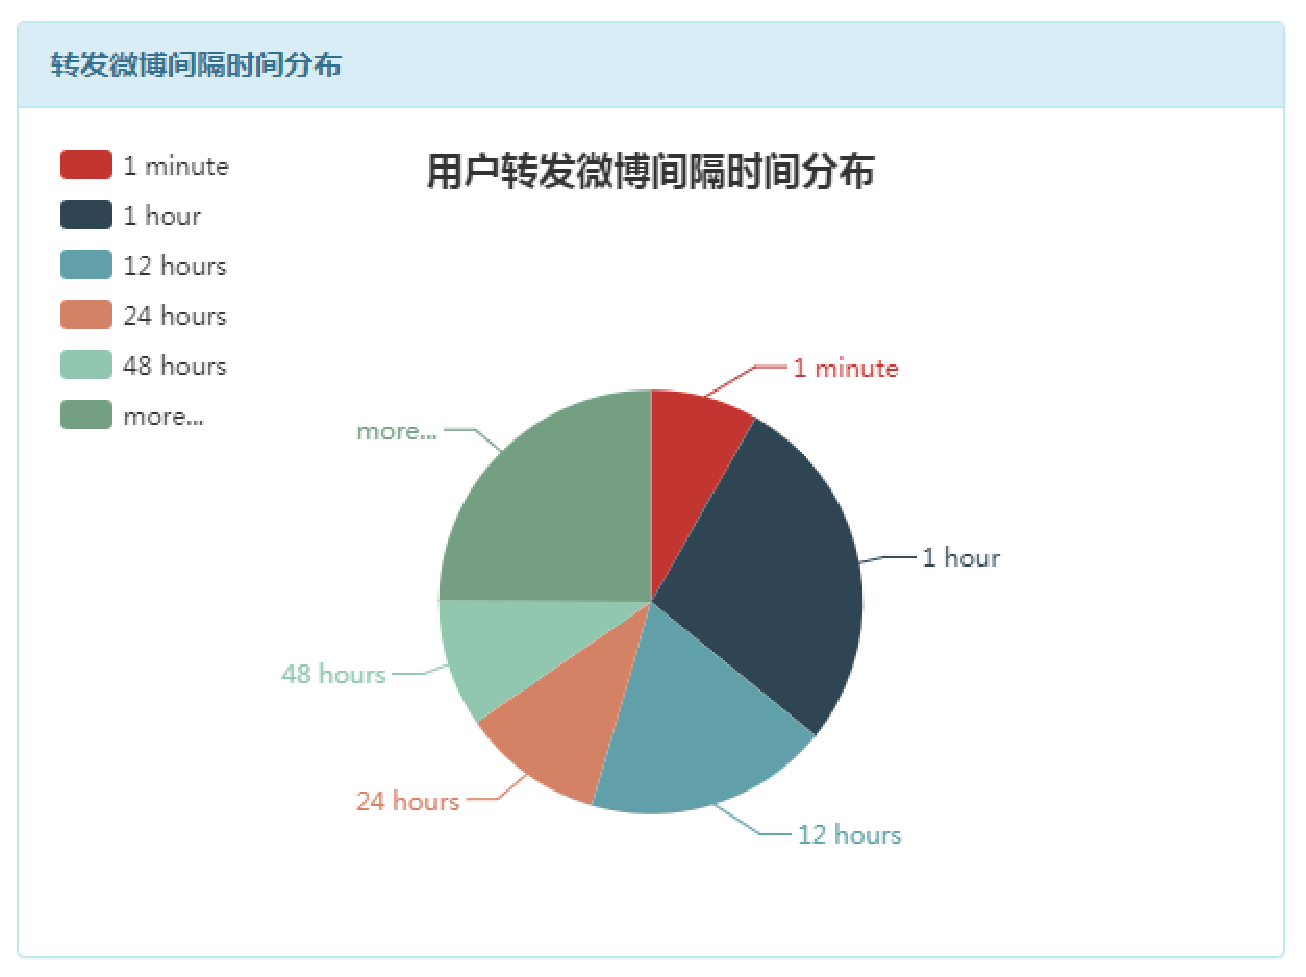
\includegraphics[width=0.15\textwidth]{IMAGE/group-images/38.eps}}
  \subfigure{
      
\includegraphics[width=0.15\textwidth]{IMAGE/group-images/39.eps}}
  \caption{The Statistics of User Group Three}
  \label{fig:subfig3} %% label for entire figure
\end{figure}
\begin{figure}
  \centering
  \subfigure{
      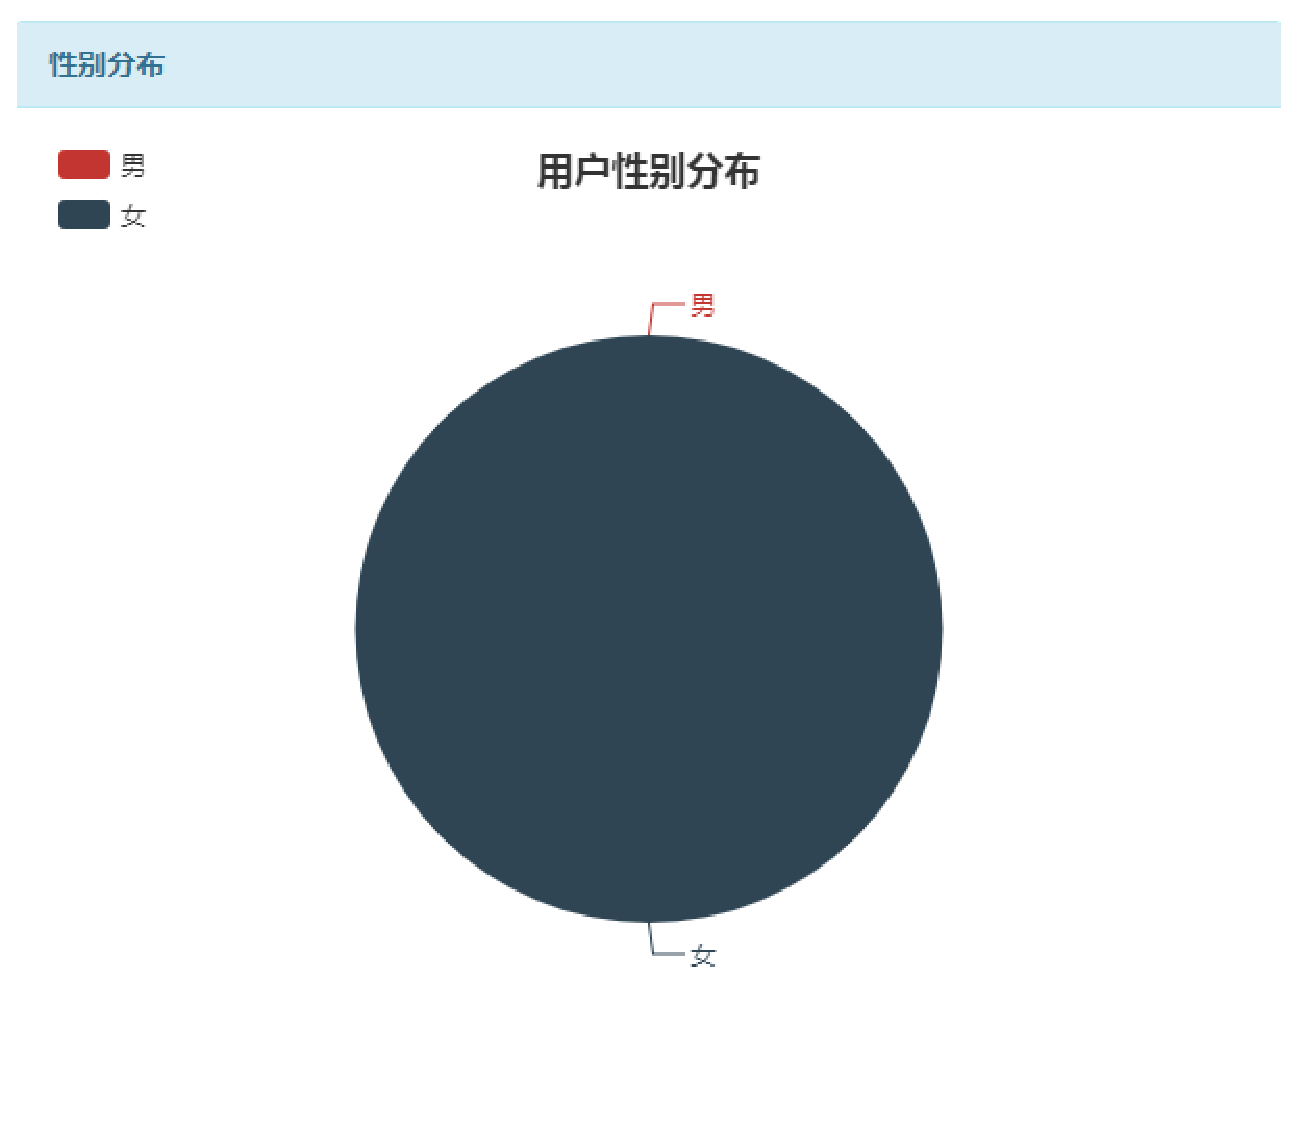
\includegraphics[width=0.15\textwidth]{IMAGE/group-images/41.eps}}
  \subfigure{
      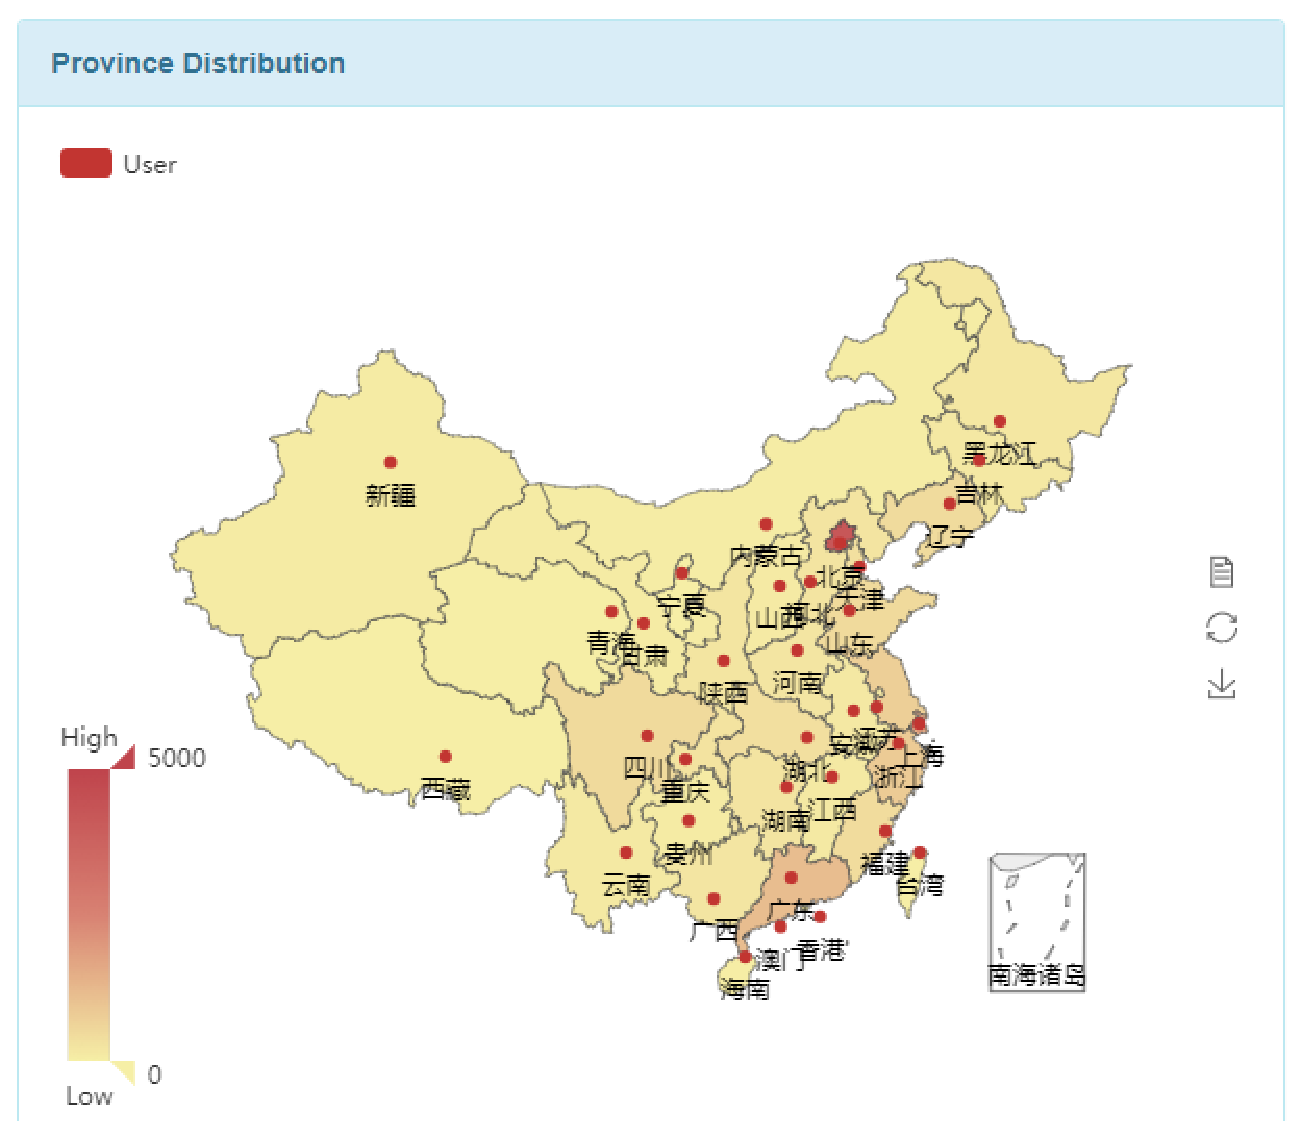
\includegraphics[width=0.15\textwidth]{IMAGE/group-images/42.eps}}
  \subfigure{
      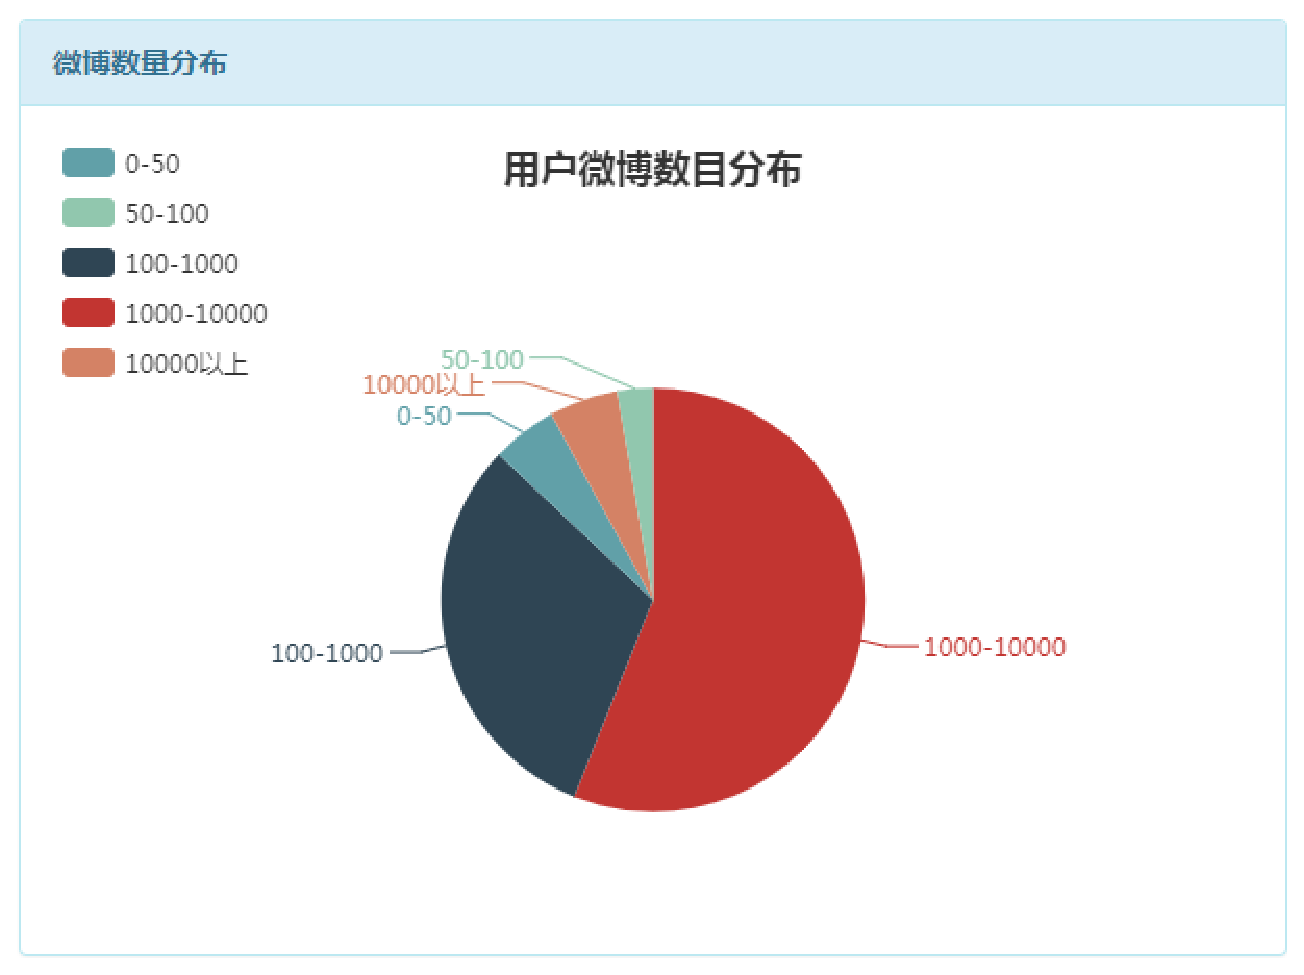
\includegraphics[width=0.15\textwidth]{IMAGE/group-images/43.eps}}
  \subfigure{
      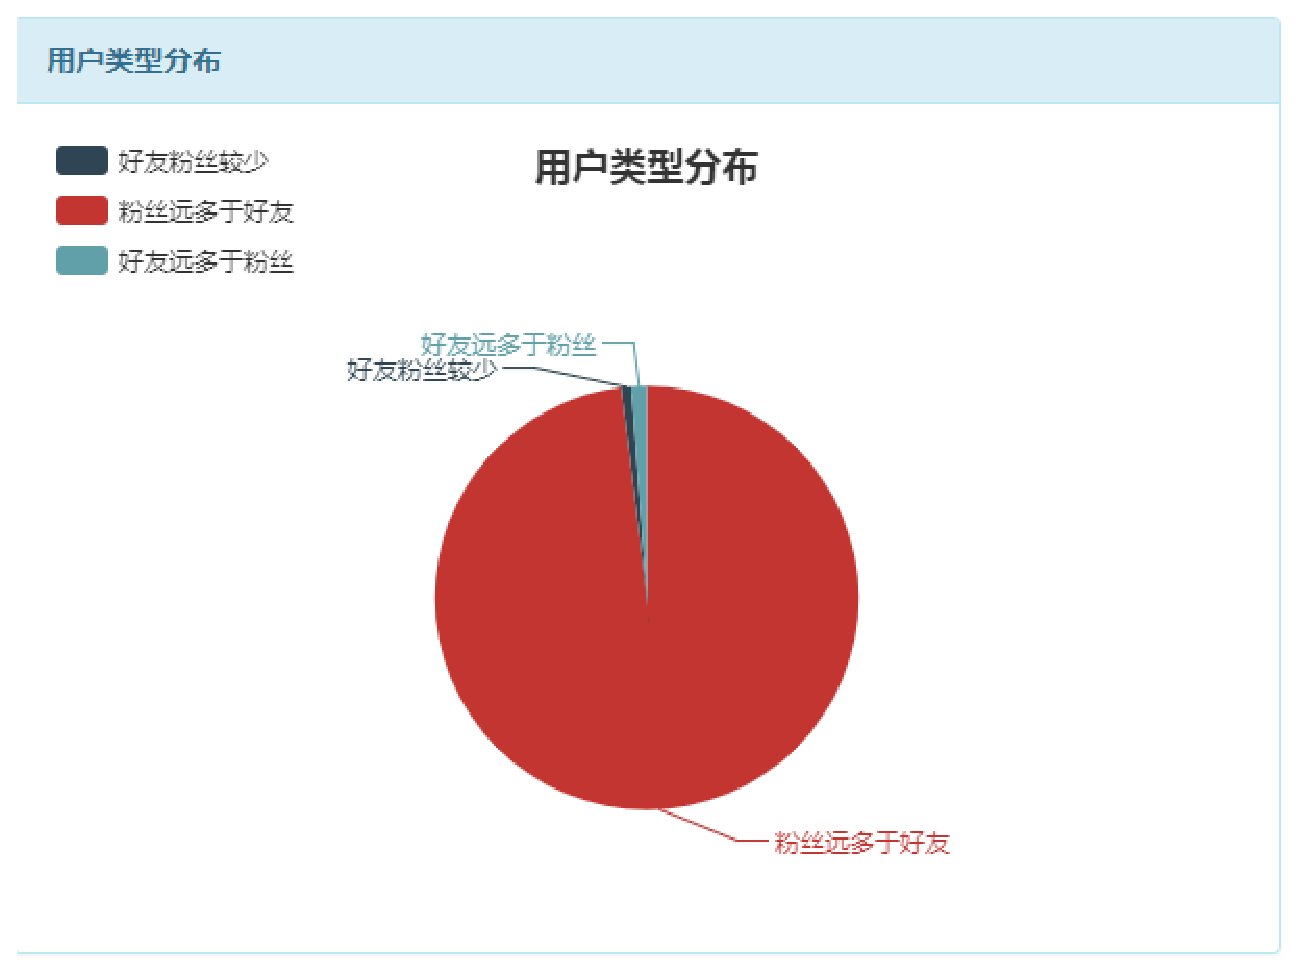
\includegraphics[width=0.15\textwidth]{IMAGE/group-images/44.eps}}
  \subfigure{
      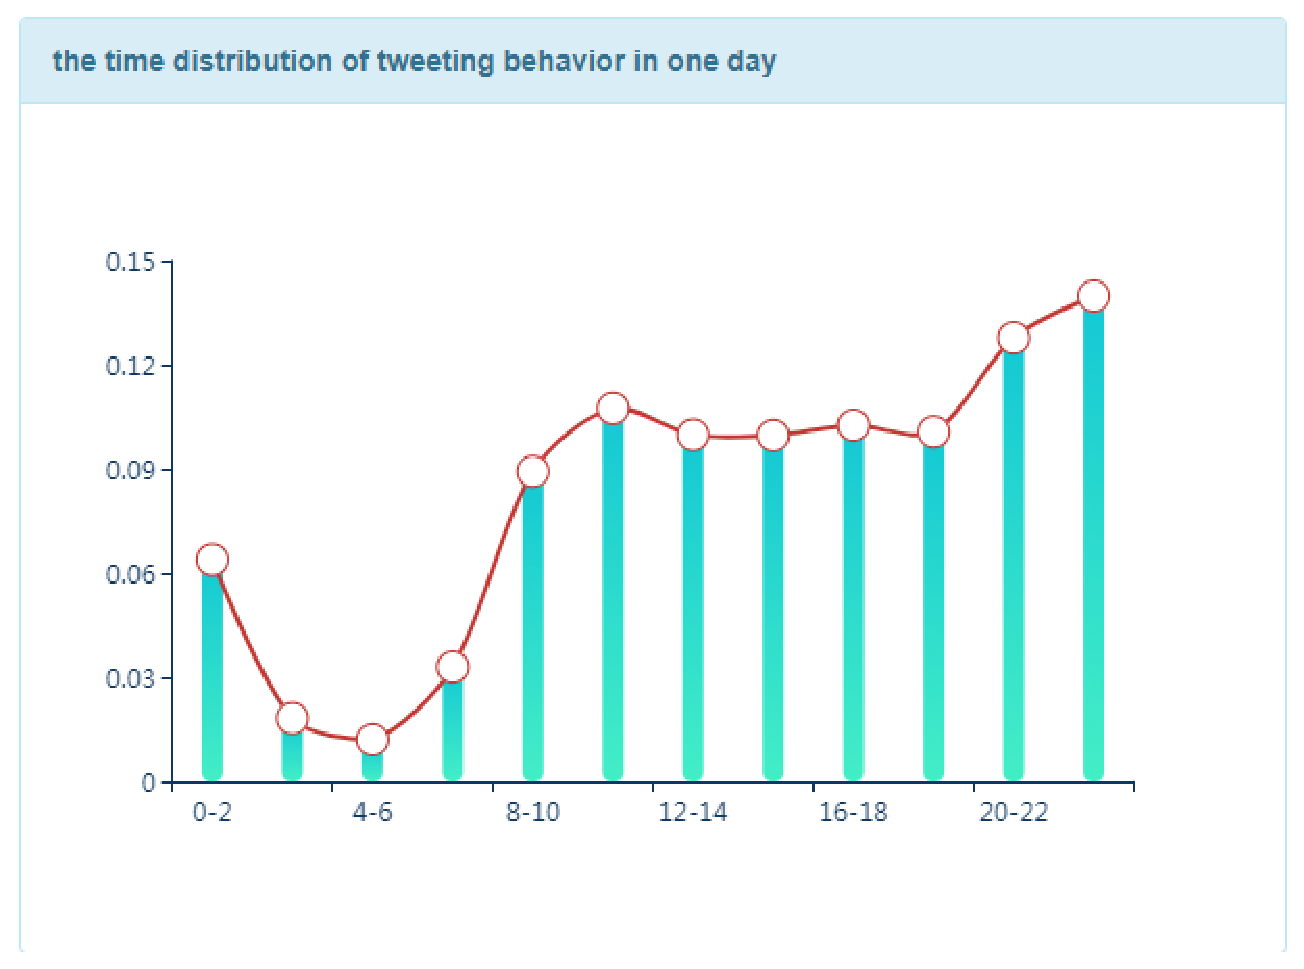
\includegraphics[width=0.15\textwidth]{IMAGE/group-images/45.eps}}
  \subfigure{
      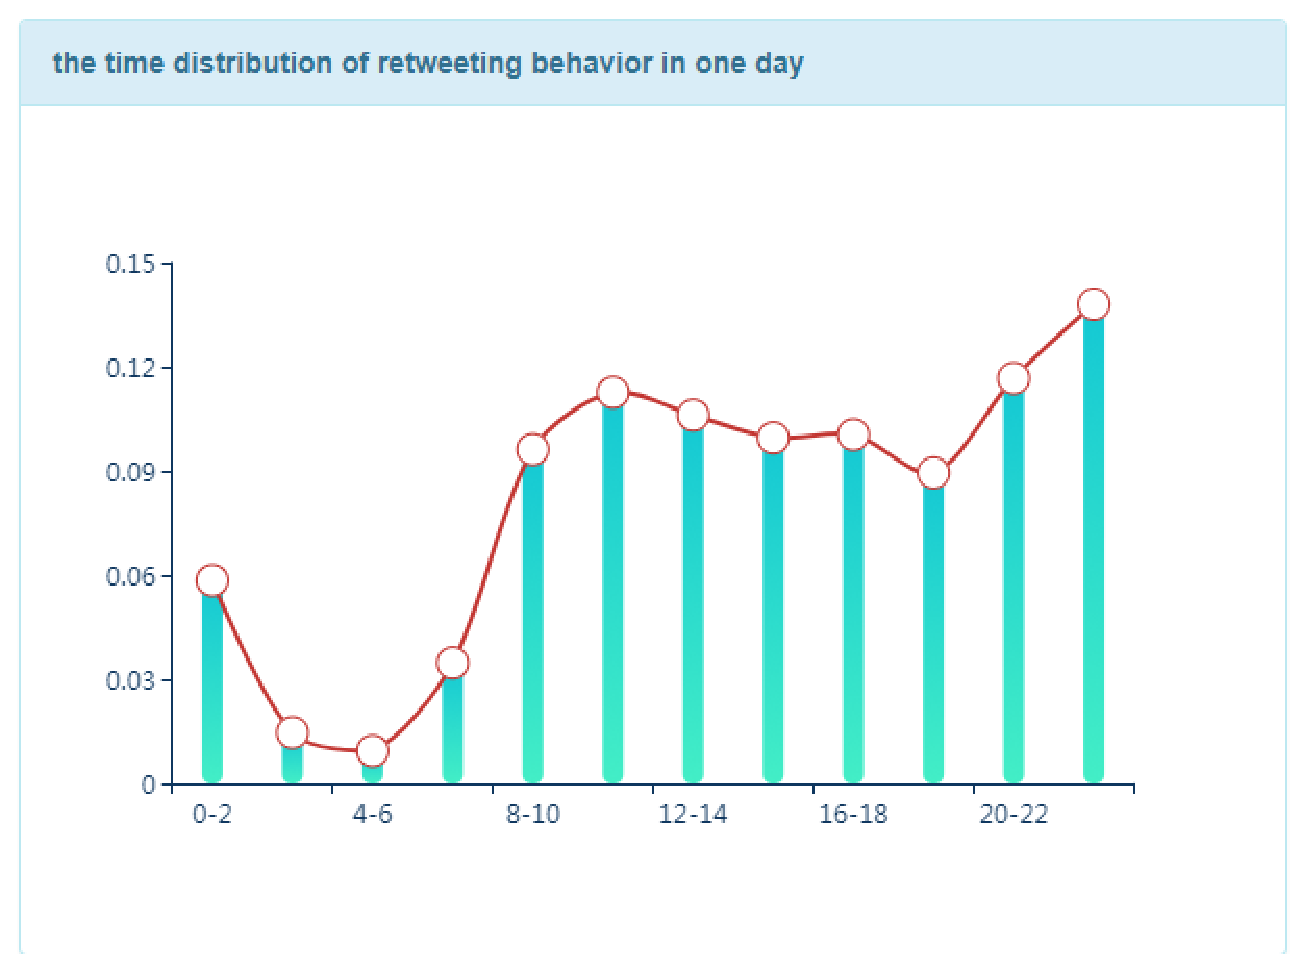
\includegraphics[width=0.15\textwidth]{IMAGE/group-images/46.eps}}
  \subfigure{
      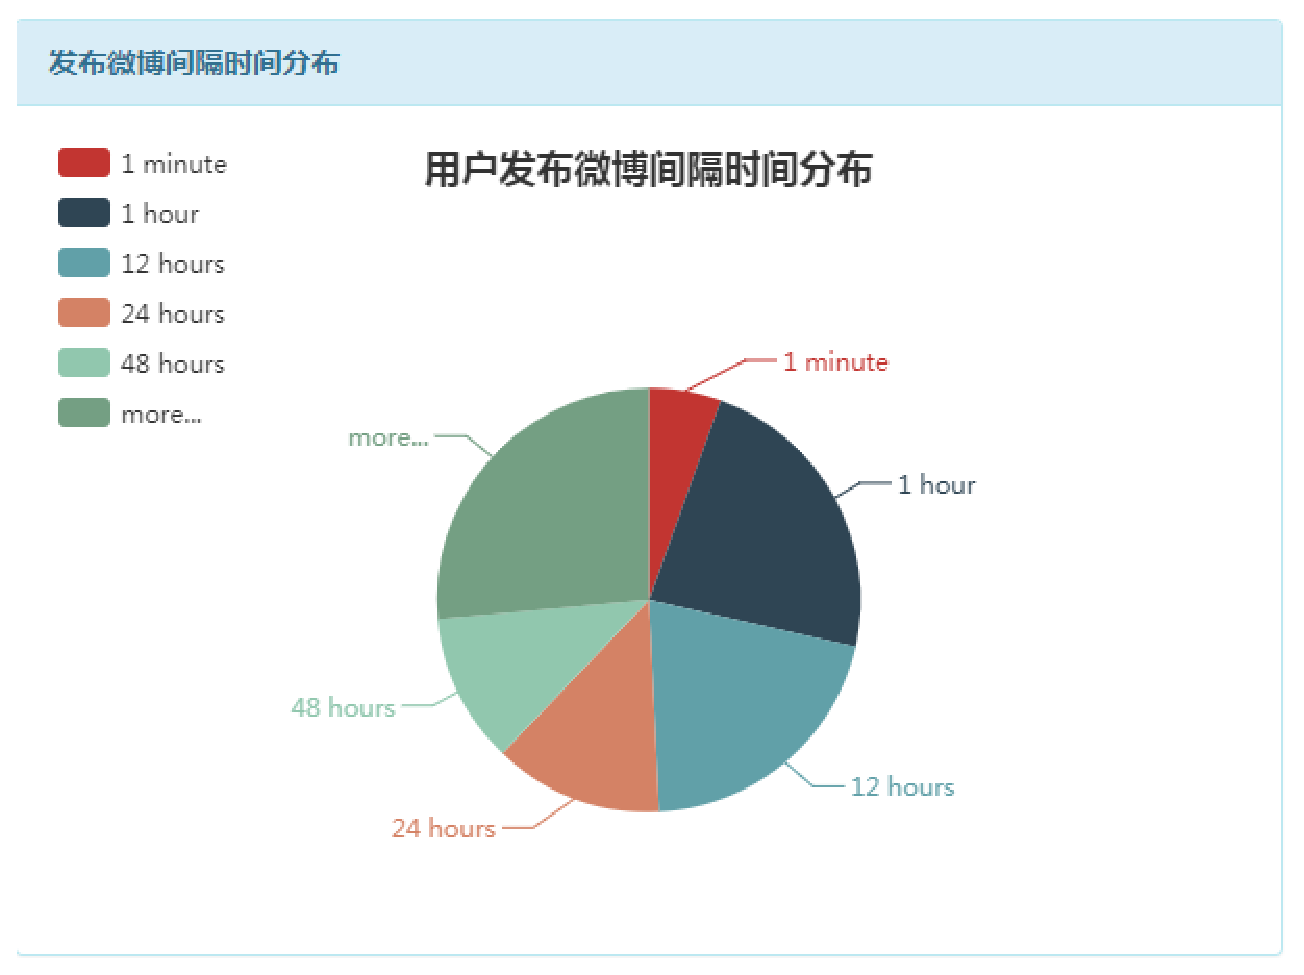
\includegraphics[width=0.15\textwidth]{IMAGE/group-images/47.eps}}
  \subfigure{
      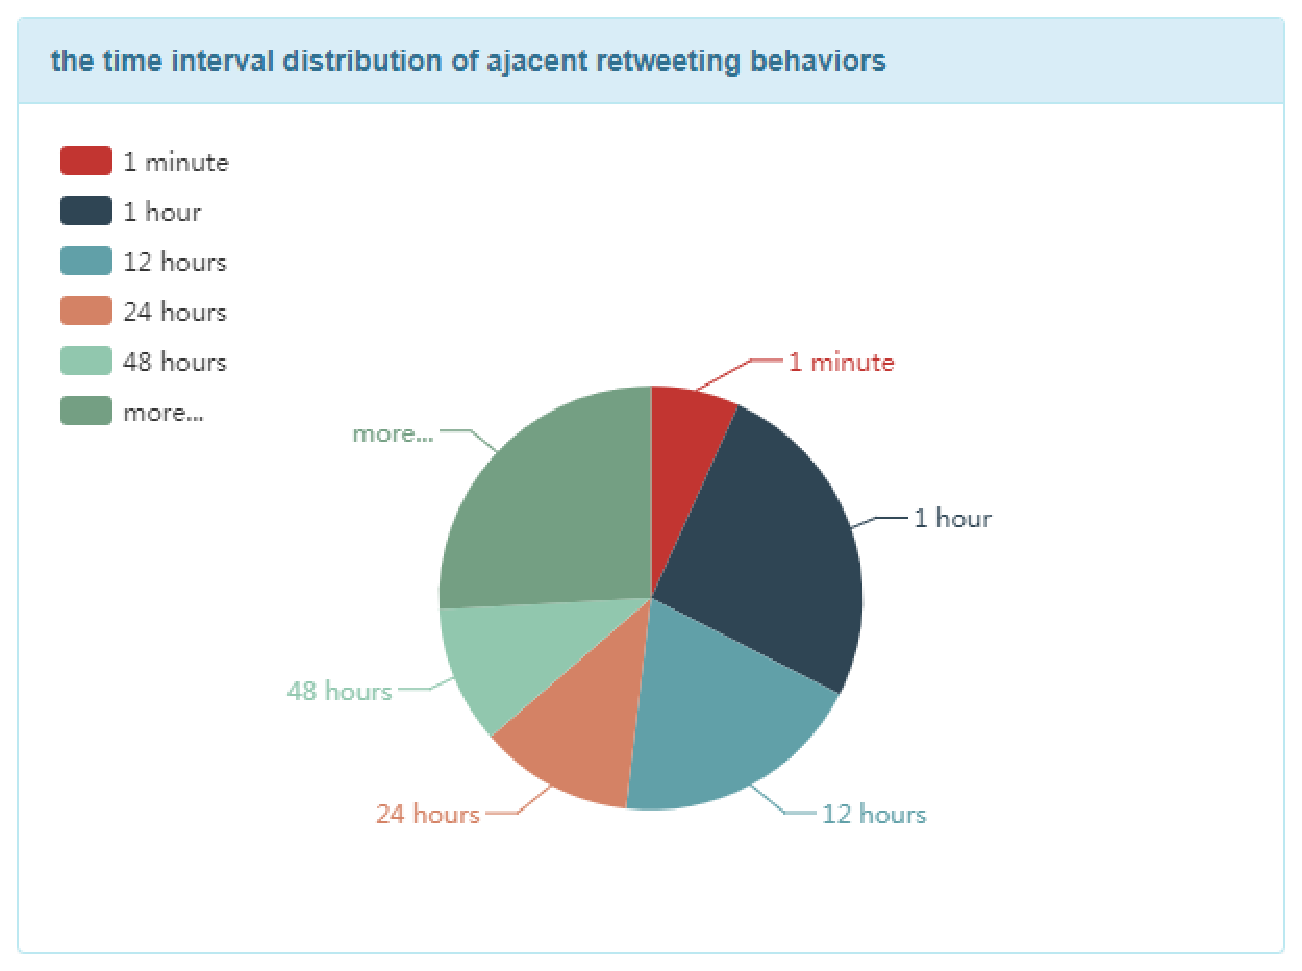
\includegraphics[width=0.15\textwidth]{IMAGE/group-images/48.eps}}
  \subfigure{
      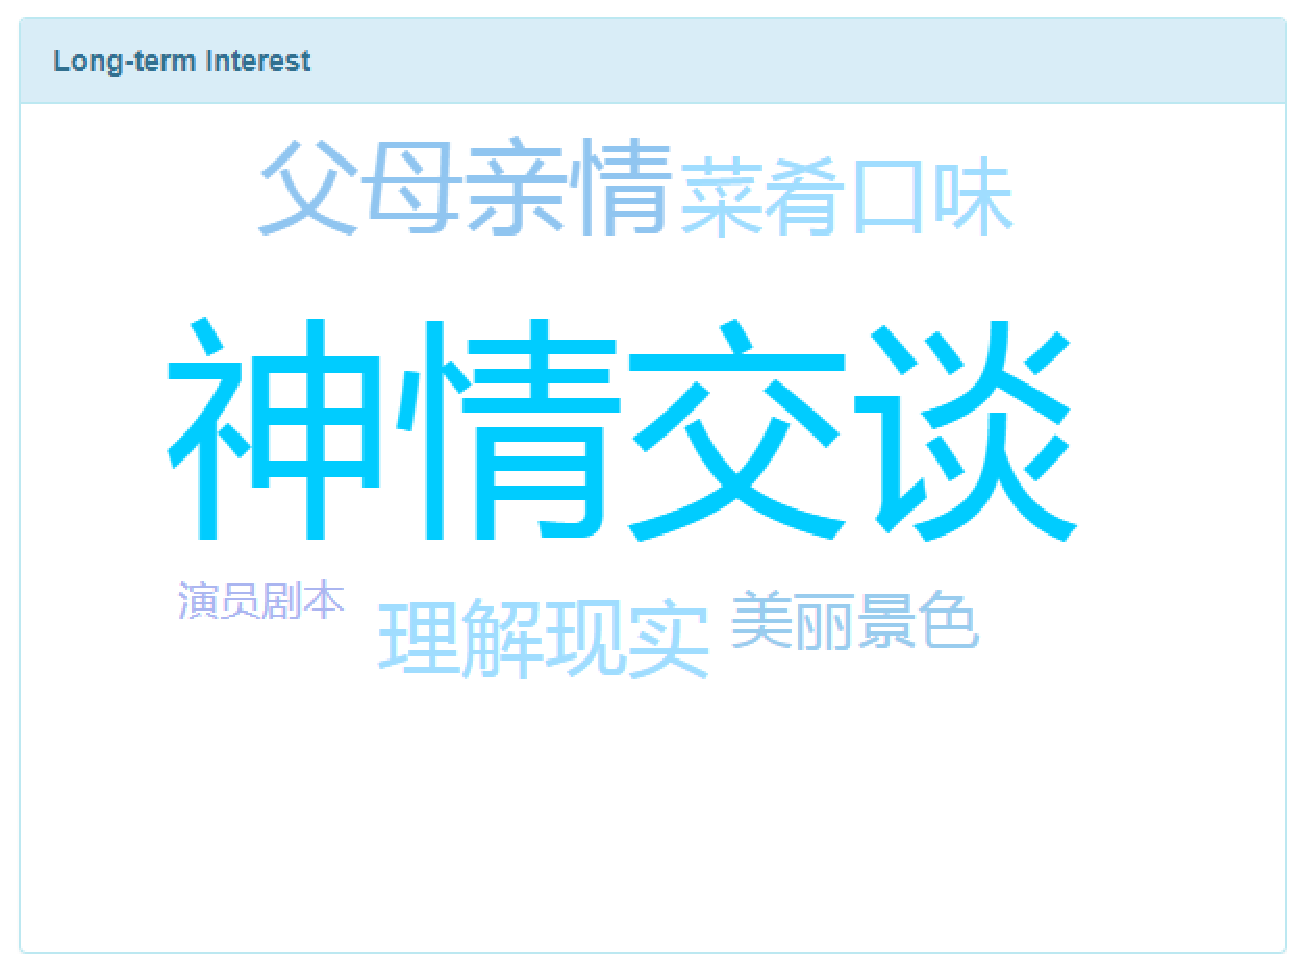
\includegraphics[width=0.15\textwidth]{IMAGE/group-images/49.eps}}
  \caption{The Statistics of User Group Four}
  \label{fig:subfig4} %% label for entire figure
\end{figure}
